\documentclass{beamer}
\usepackage[english]{babel}
\usepackage[latin1]{inputenc}
\usepackage{times}
\usepackage[T1]{fontenc}
\usepackage{lmodern}
\usepackage{underscore}
\usepackage{tikz}
\usepackage[absolute,overlay]{textpos}
\usepackage{upquote} % for single quotes in verbatim environments 
\usepackage{textcomp} % to display correctly single quotes inside verbatim
\setlength{\TPHorizModule}{1cm}
\setlength{\TPVertModule}{1cm}

% Copyright 2016-2022 Istituto Nazionale di Fisica Nucleare (INFN)

\newenvironment<>{codeblock}{%
  \begin{actionenv}#1%
    \def\insertblocktitle{}%
    \par%
    \mode<presentation>{%\usebeamerfont{block}%
      \setbeamercolor{local structure}{parent=example text}}%
    \usebeamertemplate{block example begin}%
    \begin{semiverbatim}}
                 {\par%
                   \end{semiverbatim}%
                   \usebeamertemplate{block example end}%
                 \end{actionenv}}

\mode<presentation>
{
  \usetheme{default}

  \setbeamerfont{block body example}{size=\scriptsize}
  \setbeamertemplate{blocks}[rounded][shadow=false]
  \setbeamertemplate{itemize item}[circle]
  \setbeamertemplate{itemize subitem}{$\circ$}
  \setbeamertemplate{itemize subsubitem}{$-$}
  \addtobeamertemplate{navigation symbols}{}{%
	  \usebeamerfont{footline}%
	  \usebeamercolor[fg]{footline}%
		\hspace{1em}%
		\insertframenumber
	}
  \usecolortheme{whale} % applies to outer elements
  \setbeamercolor*{block body example}{use={frametitle,normal text},fg=normal text.fg,bg=frametitle.bg!5!white}
}

% Or whatever. Note that the encoding and the font should match. If T1
% does not look nice, try deleting the line with the fontenc.

%\DisableLigatures{encoding = T1, family = tt*}

\renewcommand{\~}{\protect\scalebox{1.2}{\textasciitilde}}
\newcommand{\code}[1]{\texttt{#1}}
\newcommand{\bslash}{\textbackslash}
\newcommand\upquote[1]{\textquotesingle#1\textquotesingle}
\newcommand{\bslashn}{\upquote{\bslash{}n}}
\newcommand{\opt}[1]{#1\ensuremath{_{\mathit{opt}}}}
\newcommand{\ddd}{\(\cdots\)}

\usetikzlibrary{arrows.meta}
\usetikzlibrary{shapes.arrows}

\tikzset{
  memory/.style={rectangle,draw=black!50,minimum width=.9\textwidth,minimum height=.5cm},
  word/.style={rectangle,minimum width=1.cm,minimum height=.5cm,fill=green!20!white,draw=black!50},
  phantom word/.style={rectangle,minimum width=1.cm,minimum height=.5cm},
  word anchor/.style={rectangle,minimum width=0.25cm,minimum height=0.5cm,draw=black,densely dotted}
}

\title{Efficient C++ Programming\\ and Memory Management}

\author{F.~Giacomini}

\institute{INFN-CNAF}

\date{ESC22 --- Bertinoro, 3--8 October 2022}

\AtBeginSection[] % Do nothing for \section*
{
  \begin{frame}<beamer>
    \frametitle{Outline}
    \tableofcontents[currentsection]
  \end{frame}
}

\begin{document}

% !TeX root = cpp-esc22.tex

\begin{frame}
   \begin{tikzpicture}[remember picture,overlay]
     \node at ([yshift=-1.5cm]current page.north) {
\includegraphics[height=1.6cm]{images/logo_esc}};
     \node at ([yshift=2cm]current page.south) {\tiny\url{https://github.com/giacomini/cpp-memory-esc22}};
     \node at ([yshift=1cm]current page.south) {
\includegraphics[height=.5cm]{images/by-sa}};
   \end{tikzpicture}
   \titlepage
\end{frame}

\begin{frame}{Outline}
  \tableofcontents
  % You might wish to add the option [pausesections]
\end{frame}

% !TeX root = cpp-esc22.tex

\section{Introduction}

\begin{frame}{What is C++}
  C++ is a complex and large programming language (and library)
  \begin{itemize}[<+->]
    \item strongly and statically typed
    \item general-purpose
    \item multi-paradigm
    \item good from low-level programming to high-level abstractions
    \item efficient (\textit{``you don't pay for what you don't use''})
    \item standard
  \end{itemize}

\end{frame}

\begin{frame}{Learn more}
  \begin{itemize}
    \item Start from
      \begin{itemize}
      \item \url{https://isocpp.org/}
      \item \url{https://cppreference.com/}
      \item \url{https://github.com/isocpp/CppCoreGuidelines}
      \end{itemize}
    \item Main C++ conferences
      \begin{itemize}
      \item \url{https://github.com/cppcon}, \url{https://youtube.com/cppcon}
      \item \url{https://github.com/boostcon}, \url{https://youtube.com/boostcon}
      \end{itemize}
  \end{itemize}
\end{frame}

\begin{frame}{Standards}

  \begin{itemize}

  \item A new standard is published every three years.

  \item \textit{Working drafts}, almost the same as the final published document
    \begin{description}
    \item [C++03] \url{https://wg21.link/n1905}
    \item [C++11] \url{https://wg21.link/std11}
    \item [C++14] \url{https://wg21.link/std14}
    \item [C++17] \url{https://wg21.link/std17}
    \item [C++20] \url{https://wg21.link/std20}
    \item [C++2b] \url{https://wg21.link/std} (current draft)
    \end{description}

    \LaTeX sources at \url{https://github.com/cplusplus/draft}

  \item \textit{Working papers} at {\footnotesize
    \url{http://www.open-std.org/jtc1/sc22/wg21/docs/papers/}}

  \end{itemize}

\end{frame}

\begin{frame}{Compilers}
  \begin{itemize}
  \item The ESC machines provide many compilers: use gcc 9.2, possibly in C++17 mode (see instructions on how to enable
  it)
  \item You can also edit and try your code online with multiple compilers at
    \begin{itemize}
    \item \url{https://godbolt.org/}
    \item \url{https://coliru.stacked-crooked.com/}
    \item \url{https://wandbox.org/}
    \item \url{https://repl.it/}
    \end{itemize}
  \end{itemize}
\end{frame}

% !TeX root = cpp-esc22.tex

\section{Algorithms and functions}

\begin{frame}{The C++ standard library}

  \begin{itemize}[<+->]
  \item The standard library contains components of general use
    \begin{itemize}[<.->]
    \item \alert<2>{containers (data structures)}
    \item \alert<2>{algorithms}
    \item strings
    \item input/output
    \item random numbers
    \item regular expressions
    \item concurrency and parallelism
    \item filesystem
    \item ...
    \end{itemize}

  \item The subset containing containers and algorithms is
    known as STL (Standard Template Library)
  \item But templates are everywhere
  \end{itemize}

\end{frame}

\begin{frame}{STL Algorithms}

  \begin{itemize}[<1->]
  \item Generic functions that operate on \alert{ranges} of objects
  \item Implemented as function templates
  \end{itemize}

  \pause

  \begin{description}[<+->]
    \item[Non-modifying] \code{all\_of any\_of for\_each
      count count\_if mismatch equal find find\_if adjacent\_find search ...}
    \item[Modifying] \code{copy fill generate transform remove
      replace swap reverse rotate shuffle sample unique ...}
    \item[Partitioning] \code{partition stable\_partition ...}
    \item[Sorting] \code{sort partial\_sort nth\_element ... }
    \item[Set] \code{set\_union set\_intersection set\_difference
      ...}
    \item[Min/Max] \code{min max minmax lexicographical\_compare
      clamp ...}
    \item[Numeric] \code{iota accumulate inner\_product partial\_sum
      adjacent\_difference ...}
  \end{description}
\end{frame}

\begin{frame}{Range}

  \begin{itemize}[<+->]
  \item A range is defined by a pair of \alert{iterators}
    [\textit{first}, \textit{last}), with \textit{last} referring to one
    past the last element in the range
    \begin{itemize}
    \item the range is \textit{half-open}
    \item \textit{first} == \textit{last} means the range is empty
    \item \textit{last} can be used to return failure
    \end{itemize}
  \item An \alert{iterator} allows to go through the elements of the associated
    range
    \begin{itemize}
    \item operations to advance, access, compare
    \item typically obtained from containers calling specific methods
    \end{itemize}
  \item An iterator is a generalization of a pointer
    \begin{itemize}
    \item it supports the same operations, possibly through overloaded operators
    \item certainly \code{* ++ -> == !=}, maybe \code{-{}- + - += -= <}
    \end{itemize}
  \item C++20 introduced \code{ranges}, a new library of \textit{concepts} and components for dealing with ranges of
    objects (not discussed here)
  \end{itemize}

\end{frame}

\begin{frame}[fragile]{Range \insertcontinuationtext}

  \begin{tikzpicture}
    [anchor=south west]
    \visible<1->{\node at (0,0) [memory] {};}
    \visible<1->{\node at (0,0) [word anchor,label={90:{\tiny\tt 0x0000}}] {};}
    \visible<1->{\node at (.9\textwidth-.25cm,0) [word anchor,label={90:{\tiny\tt 0xffff}}] {};}

    \visible<1->{\node at (3.9,-0.1) [
        rectangle,
        fill=green!10!white,
        draw=black!40,
        minimum width=3.2cm,
        minimum height=0.7cm,
        label=270:{\scriptsize\tt a},
      ] {};
    }
    \visible<1->{\node (a0) at (4,0) [word] {\scriptsize\tt\alert<5>{123}};}
    \visible<1->{\node (a1) at (5,0) [word] {\scriptsize\tt\alert<8>{456}};}
    \visible<1->{\node (a2) at (6,0) [word] {\scriptsize\tt\alert<11>{789}};}
    \visible<1->{\node (a3) at (7,0) [phantom word] {};}
    \visible<1->{\node at (4,0) [word anchor,label={90:{\tiny\tt 0xab00}}] {};}
    \visible<1->{\node at (5,0) [word anchor,label={90:{\tiny\tt 0xab04}}] {};}
    \visible<1->{\node at (6,0) [word anchor, label={90:{\tiny\tt 0xab08}}] {};}
    \visible<1->{\node at (7,0) [word anchor, label={90:{\tiny\tt0xab0c}}] {};}
    \visible<2->{\node (first) at (4,-1.5) [word, label={270:{\scriptsize\tt first}}] {};}
    \visible<3->{\node (last) at (7,-1.5) [word, label={270:{\scriptsize\tt last}}] {};}
    \visible<2-5>{\draw[->] (first.north) -- (a0.south);}
    \visible<3->{\draw[->] (last.north) --  (a3.south);}
    \visible<6-8>{\draw[->] (first.north) -- (a1.south);}
    \visible<9-11>{\draw[->] (first.north) -- (a2.south);}
    \visible<12->{\draw[->] (first.north) -- (a3.south);}

  \end{tikzpicture}

  \begin{codeblock}
\uncover<1->{std::array\invisible<16>{<int,3>} a = \{123, 456, 789\};\uncover<16>{ // \alert{CTAD}}}
\uncover<2->{\alert<2>{auto first = a.begin();}       // or std::begin(a)}
\uncover<3->{\alert<3>{auto\only<14->{\alert<14>{ const}} last = a.end();}\only<-13>{      }    // or std::end(a)}
\uncover<4->{while (\alert<4,7,10,13>{first != last}) \{       // comparison
  ... \alert<5,8,11>{*first} ...;             // access
  \alert<6,9,12>{++first};                    // advance
\}}\end{codeblock}

  \begin{itemize}[<15->]
  \item \code{std::array<T>::iterator} models the \textit{RandomAccessIterator} concept
  \end{itemize}
\end{frame}

\begin{frame}[fragile]{Generic programming}

  \begin{itemize}[<+->]
  \item A style of programming in which \alert{algorithms} are written
    in terms of \alert{concepts}

  \begin{codeblock}<+->
template <class Iterator, class T>
Iterator
find(Iterator first, Iterator last, const T\& value)
\{
  for (; first \alert{!=} last; \alert{++}first)
    if (\alert{*}first \alert{==} value)
      break;
  return first;
\}\end{codeblock}

  \item A concept is a set of requirements that a type needs to satisfy
    \begin{itemize}[<.->]
    \item e.g. supported expressions, nested types, memory layout, \ldots
    \end{itemize}
  \end{itemize}


\end{frame}

\begin{frame}[fragile]{Range \insertcontinuationtext}

  \begin{tikzpicture}
    [anchor=south west]
    \visible<1->{\node at (0,0) [memory] {};}
    \visible<1->{\node at (0,0) [word anchor,label={90:{\tiny\tt 0x0000}}] {};}
    \visible<1->{\node at (.9\textwidth-.25cm,0) [word anchor,label={90:{\tiny\tt 0xffff}}] {};}

    \visible<1->{\node (l) at (0.9,-0.1) [
        rectangle,
        fill=green!10!white,
        draw=black!40,
        minimum width=1.2cm,
        minimum height=0.7cm,
        label=270:{\scriptsize\tt l},
      ] {};
    }
    \visible<1->{\node (a0) at (3.5,0) [word] {\scriptsize\tt\alert<5>{123}};}
    \visible<1->{\node (a1) at (6.5,0) [word] {\scriptsize\tt\alert<8>{456}};}
    \visible<1->{\node (a2) at (5  ,0) [word] {\scriptsize\tt\alert<11>{789}};}
    \visible<1->{\node (a3) at (8  ,0) [phantom word,draw=black,densely dotted] {};}
    \visible<1->{\node (c0) at (3.5,0) [word anchor,label={90:{\tiny\tt 0xab00}}] {};}
    \visible<1->{\node (c1) at (6.5,0) [word anchor,label={90:{\tiny\tt 0xad08}}] {};}
    \visible<1->{\node (c2) at (5,0) [word anchor, label={90:{\tiny\tt 0xac04}}] {};}
    \visible<1->{\node (c3) at (8,0) [word anchor] {};}
    \visible<1->{\draw[Circle-Stealth,black!50] (l.east) .. controls +(1,1) .. (c0.north);}
    \visible<1->{\draw[Circle-Stealth,black!50] (a0.east) .. controls +(1,1.5) .. (c1.north);}
    \visible<1->{\draw[Circle-Stealth,black!50] (a1.east) .. controls +(-1,1) .. (c2.north);}
    \visible<1->{\draw[Circle-Stealth,black!50] (a2.east) .. controls +(1,1.5) .. (c3.north);}
    %    \visible<1->{\node at (3,0) [word anchor,label={90:{\tiny\tt 0xab00}}] {};}
    \visible<2->{\node (first) at (3.5,-1.5) [word, label={270:{\scriptsize\tt first}}] {};}
    \visible<3->{\node (last) at (8,-1.5) [word, label={270:{\scriptsize\tt last}}] {};}
    \visible<2-5>{\draw[->] (first.north) -- (a0.south);}
    \visible<3->{\draw[->] (last.north) --  (a3.south);}
    \visible<6-8>{\draw[->] (first.north) -- (a1.south);}
    \visible<9-11>{\draw[->] (first.north) -- (a2.south);}
    \visible<12->{\draw[->] (first.north) -- (a3.south);}

  \end{tikzpicture}

  \begin{codeblock}
\uncover<1->{std::forward\_list<int> l = \{123, 456, 789\};}
\uncover<2->{\alert<2>{auto first = l.begin();}}
\uncover<3->{\alert<3>{auto const last = l.end();}}
\uncover<4->{while (\alert<4,7,10,13>{first != last}) \{
  ... \alert<5,8,11>{*first} ...;
  \alert<6,9,12>{++first};
\}}\end{codeblock}

  \begin{itemize}[<14->]
  \item \code{std::forward\_list<T>::iterator} models the \textit{ForwardIterator} concept
  \end{itemize}
\end{frame}

\begin{frame}[fragile]{Algorithms and ranges}

  \begin{itemize}
  \item Examples
    \begin{codeblock}
std::vector v = \{ 23, 54, 41, 0, 18 \};

// sort the vector in ascending order
std::sort(std::begin(v), std::end(v));

// sum up the vector elements, initializing the sum to 0
auto s = std::accumulate(std::begin(v), std::end(v), 0);
auto r = std::reduce(std::begin(v), std::end(v));

// append the partial sums of the vector elements into a list
std::list<int> l;
std::partial\_sum(std::begin(v), std::end(v), std::back\_inserter(l));

// find the first element with value 42
auto it = std::find(std::begin(v), std::end(v), 42);
    \end{codeblock}

  \item Some algorithms are customizable passing a function
    \begin{codeblock}
auto it = std::find_if(v.begin(), v.end(), \alert{\textit{filter}});\end{codeblock}
  \end{itemize}
\end{frame}

\begin{frame}{Hands-on}
  \begin{itemize}
  \item C++ $\rightarrow$ Algorithms
  \item Starting from \code{algo.cpp} and following the hints, write code to
    \begin{itemize}
    \item sum all the elements of the vector
    \item compute the average of the first half and of the second half of the
      vector
    \item move the three central numbers to the beginning
    \item remove duplicate elements
    \item \ldots
    \end{itemize}
  \end{itemize}
\end{frame}

\begin{frame}[fragile]{Why using standard algorithms}

  \begin{itemize}[<+->]
  \item They are correct
  \item They express intent more clearly than a raw \code{for} loop
  \item They enable \textit{parallelism for the masses}
    \begin{itemize}[<.->]
    \item parallel algorithms available in C++17, implementations are appearing
    \end{itemize}
  \end{itemize}

  \begin{codeblock}<+->{
#include <execution>

std::vector<int> v = \ddd;
std::sort(\alert{std::execution::par}, v.begin(), v.end());
auto it = std::find(\alert{std::execution::par}, v.begin(), v.end(), 42);}\end{codeblock}

\end{frame}

\begin{frame}{Hands-on}
  \begin{itemize}
  \item C++ $\rightarrow$ Algorithms
  \item Starting from \code{algo\_par.cpp} and following the hints, write code to
    \begin{itemize}
    \item sum all the elements of the vector, with and without parallelization
    \item sort the vector, with and without parallelization
    \item \ldots
    \end{itemize}
    and compare the execution times.
  \end{itemize}
\end{frame}

\begin{frame}[fragile]{Functions}

  \begin{itemize}
  \item<1-> A function associates a sequence of statements (the function
    \textit{body}) with a name and a list of zero or more parameters

  \begin{codeblock}<2->
\alt<2>{std::string}{\alert<3>{auto        }} join(std::string const\& s, int i)
\{
  return s + \upquote{-} + std::to\_string(i);
\}

join("XYZ", 5); // std::string\{"XYZ-5"\}\end{codeblock}

  \item<4-> A function may return a value
  \item<5-> A function returning a \code{bool} is called a \textit{predicate}
    \begin{codeblock}
\alert<5>{bool} less(int n, int m) \{ return n < m; \}\end{codeblock}

  \item<6-> Multiple functions can have the same name $\rightarrow$
    \textit{overloading}
    \begin{itemize}
    \item different parameter lists
    \end{itemize}
  \end{itemize}

\end{frame}

\begin{frame}[fragile]{Algorithms and functions}

  \begin{codeblock}{\tiny
template <class Iterator, class T>
Iterator find(Iterator first, Iterator last, \alert{const T\& value})
\{
  for (; first != last; ++first)
    if (\alert{*first == value})
      break;
  return first;
\}

auto it = find(v.begin(), v.end(), 42);}\end{codeblock}

  \begin{codeblock}<2->
template <class Iterator, class T>
Iterator find_if(Iterator first, Iterator last, \alert{T pred})
\{
  for (; first != last; ++first)
    if (\alert{pred(*first)})          // unary predicate
      break;
  return first;
\}

\uncover<3->{bool lt42(int n) \{ return n < 42; \}}

\uncover<4->{auto it = find_if(v.begin(), v.end(), lt42);}\end{codeblock}

\end{frame}

\begin{frame}[fragile]{Function objects}

  A mechanism to define \textit{something-callable-like-a-function}
  \begin{itemize}
  \item<4-> A class with an \texttt{operator()}
  \end{itemize}

  \begin{columns}[t]

    \begin{column}{.5\textwidth}

      \begin{codeblock}<2->{
\invisible{struct LessThan42 \{}
auto \alert<2,4>{lt42}(int n)
\{
  return n < 42;
\}

\invisible{
LessThan42 lt42\{\};}
auto b = \alert<2,7>{lt42(}32\alert<2,7>{)}; // true

\uncover<3->{vector v\{61,32,51\};
auto it = find_if(
    begin(v), end(v),
    \alert<3,8>{lt42}
); // *it == 32}}\end{codeblock}

    \end{column}

    \begin{column}{.5\textwidth}

      \begin{codeblock}<4->{
\alert<4>{struct LessThan42 \{}
  auto \alert<4>{operator()}(int n) \alert<4>{const}
  \{
    return n < 42;
  \}
\alert<4>{\};}

\uncover<5->{\alt<5>{LessThan42 lt42\{\};}{auto lt42 = LessThan42\{\};}}
\uncover<7->{auto b = \alert<7>{lt42(}32\alert<7>{)}; // true}

\uncover<8,9>{vector v\{61,32,51\};
auto it = find_if(
    begin(v), end(v),
    \alert{\alt<8>{lt42}{LessThan42\{\}}}
); // *it == 32}}\end{codeblock}

    \end{column}
  \end{columns}
\end{frame}

\begin{frame}[fragile]{Function objects \insertcontinuationtext}
  A function object, being the instance of a class, can have state
  \begin{codeblock}<2->{
class LessThan \{
  \alert<2>{int m\_;}
 public:
  explicit \alert<2>{LessThan(int m) : m\_\{m\} \{\}}
  auto operator()(int n) const \{
    return n < m_;
  \}
\};

\uncover<3->{auto lt42 = LessThan\{42\};
auto b1 = \alt<-5>{lt42}{\alert<6>{LessThan\{42\}}}(32); // true}

\uncover<4->{auto lt24 = LessThan\{24\};
auto b2 = \alt<-5>{lt24}{\alert<6>{LessThan\{24\}}}(32); // false}

\uncover<5->{vector v\{61,32,51\};
auto i1 = find_if(\ldots, \alt<-5>{lt42}{\alert<6>{LessThan\{42\}}}); // *i1 == 32
auto i2 = find_if(\ldots, \alt<-5>{lt24}{\alert<6>{LessThan\{24\}}}); // i2 == end, i.e. not found}}\end{codeblock}

  \uncover<6>{}

\end{frame}

\begin{frame}[fragile]{Function objects \insertcontinuationtext}
  An example from the standard library

  \begin{codeblock}
#include <random>

// random bit generator
std::default_random_engine gen;

// generate N 32-bit unsigned integer numbers
for (int n = 0; n != N; ++n) \{
  std::cout <{}< \alert{gen()} <{}< \bslashn;
\}

// generate N floats distributed normally (mean: 0., stddev: 1.)
std::normal_distribution<float> dist;
for (int n = 0; n != N; ++n) \{
  std::cout <{}< \alert{dist(gen)} <{}< \bslashn;
\}

// generate N ints distributed uniformly between 1 and 6 included
std::uniform\_int\_distribution<> roll\_dice(1, 6);
for (int n = 0; n != N; ++n) \{
  std::cout <{}< \alert{roll\_dice(gen)} <{}< \bslashn;
\}\end{codeblock}

\end{frame}

\begin{frame}[fragile]{Lambda expression}

  \begin{itemize}
  \item A concise way to create an unnamed function object
  \item Useful to pass actions/callbacks to algorithms, threads, frameworks,
    \ldots
  \end{itemize}

  \begin{columns}[t]

    \begin{column}{.5\textwidth}
      \begin{codeblock}<2->{
struct LessThan42 \{
  auto operator()(int n)
  \{
    return n < 42;
  \}
\};

class LessThan \{
  int m\_;
 public:
  explicit LessThan(int m)
    : m\_\{m\} \{\}
  auto operator()(int n) const
  \{
    return n < m_;
  \}
\};}\end{codeblock}

    \end{column}

    \begin{column}{.5\textwidth}
      \begin{codeblock}<2->{
find_if(\ldots, LessThan42\{\});

\uncover<3->{find_if(\ldots, \alert<3>{[](int n) \{}
               return n < 42;
             \alert<3>{\}}
);}

find_if(\ldots, LessThan\{42\});

\uncover<4->{\only<4>{\alert{int m\{42\};}}
find_if(\ldots, [\alert<4->{\only<4>{=}\only<5>{m = 42}}](int n) \{
              return n < \alert<4->{m};
             \}
);}}\end{codeblock}
    \end{column}

  \end{columns}
\end{frame}

\begin{frame}[fragile]{Lambda expression \insertcontinuationtext}
  The evaluation of a lambda expression produces an unnamed function object (a
  \textit{closure})
  \begin{itemize}
  \item The \texttt{operator()} corresponds to the code of the body of the
    lambda expression
  \item The data members are the captured local variables

    \begin{itemize}
    \item \texttt{[]} capture nothing
    \item \texttt{[=]} capture all by value
    \item \texttt{[k]} capture \texttt{k} by value
    \item \texttt{[\&]} capture all by reference
    \item \texttt{[\&k]} capture \texttt{k} by reference
    \item \texttt{[=, \&k]} capture all by value but \texttt{k} by reference
    \item \texttt{[\&, k]} capture all by reference but \texttt{k} by value
    \end{itemize}

  \item Global variables are available without being captured
  \end{itemize}
\end{frame}

\begin{frame}{Hands-on}
  \begin{itemize}
  \item C++ $\rightarrow$ Algorithms
  \item Starting from \code{algo\_functions.cpp} and following the hints, write
    code to
    \begin{itemize}
    \item multiply all the elements of the vector
    \item sort the vector in descending order
    \item move the even numbers to the beginning
    \item create another vector with the squares of the numbers in the first vector
    \item find the first multiple of 3 or 7
    \item erase from the vector all the multiples of 3 or 7
    \item \ldots
    \end{itemize}
  \end{itemize}
\end{frame}

\begin{frame}[fragile]{\texttt{std::function}}
  \begin{itemize}
  \item Type-erased wrapper that can store and invoke any callable entity with a certain signature
    \begin{itemize}
    \item function, function object, lambda, member function
    \end{itemize}
  \item Some space and time overhead, so use only if a template parameter is not satisfactory
  \end{itemize}

  \begin{codeblock}<2->{
#include <functional>
#include <iostream>

\alert{int} sum\_squares\alert{(int} x\alert{, int} y\alert{)} \{ return x * x + y * y; \}

int main() \{
  std::vector<std::function<\alert{int(int, int)}>{}> v \{
    std::plus<>\{\},       // has a compatible operator()
    std::multiplies<>\{\}, // idem
    \&sum\_squares
  \};
  for (int k = 10; k <= 1000; k *= 10) \{
    v.push\_back([k]\alert{(int} x\alert{, int} y\alert{)} -> \alert{int} \{ return k * x + y; \});
  \}
  for (auto const\& f : v) \{ std::cout <{}< f(4, 5) <{}< \bslashn; \}
\}}\end{codeblock}

\end{frame}

% !TeX root = cpp-esc22.tex

\section{Resource management}

\begin{frame}[fragile]{Weaknesses of a \texttt{T*}}

  \begin{itemize}[<+->]
  \item Critical information is not encoded in the type
    \only<.>{
      \begin{itemize}[<.>]
      \item Am I the owner of the pointee? Should I delete it?
      \item Is the pointee an object or an array of objects? of what size?
      \item Was it allocated with \texttt{new}, \texttt{malloc} or even something
        else (e.g. \texttt{fopen} returns a \texttt{FILE*})?
      \end{itemize}
    }
  \item Owning pointers are prone to leaks and double deletes
  \item Owning pointers are unsafe in presence of exceptions
  \item Runtime overhead
    \begin{itemize}
    \item<.-> dynamic allocation/deallocation
    \item<.-> indirection
    \end{itemize}
  \end{itemize}

  \begin{onlyenv}<1> % \only doesn't work for a verbatim env
    \begin{codeblock}
T* p = create\_something();\end{codeblock}
  \end{onlyenv}

  \begin{onlyenv}<2>
    \begin{codeblock}
\{
  T* p = new T\{\};
  \ddd
  // ops, forgot to delete p
\}
\{
  T* p = new T;
  \ddd
  delete p;
  \ddd
  delete p; // ops, delete again
\}\end{codeblock}
  \end{onlyenv}

  \begin{onlyenv}<3>
    \begin{codeblock}
\{
  T* p = new T;
  \ddd // potentially throwing code
  delete p;
\}\end{codeblock}
  \end{onlyenv}

\end{frame}

\begin{frame}[fragile]{Debugging memory problems}

  \begin{itemize}
  \item Valgrind is a suite of debugging and profiling tools for memory
    management, threading, caching, etc.
  \item Valgrind Memcheck can detect
    \begin{itemize}
    \item invalid memory accesses
    \item use of uninitialized values
    \item memory leaks
    \item bad frees
    \end{itemize}
  \item It's precise, but slow
  \end{itemize}

  \begin{onlyenv}<2>
    \begin{codeblock}
$ g++ leak.cpp
$ valgrind ./a.out
==18331== Memcheck, a memory error detector
...\end{codeblock}
  \end{onlyenv}

\end{frame}

\begin{frame}[fragile]{Debugging memory problems \insertcontinuationtext}

  \begin{itemize}
  \item \textit{Address Sanitizer} (ASan)
  \item The compiler instruments the executable so that at runtime ASan can
    catch problems similar, but not identical, to valgrind
  \item Faster than valgrind
  \end{itemize}

  \begin{onlyenv}<2>
    \begin{codeblock}
$ g++ -fsanitize=address leak.cpp
$ ./a.out

=================================================================
==18338==ERROR: LeakSanitizer: detected memory leaks
\ldots\end{codeblock}
  \end{onlyenv}

\end{frame}

\begin{frame}{Hands-on}
  \begin{itemize}
  \item C++ $\rightarrow$ Memory issues
  \item Get familiar with Valgrind and memory sanitizers
  \item Inspect, compile, run directly and run through valgrind or memory
    sanitizers (not both together)
    \begin{itemize}
    \item \code{non\_owning\_pointer.cpp}
    \item \code{array\_too\_small.cpp}
    \item \code{leak.cpp}
    \item \code{double\_delete.cpp}
    \item \code{missed\_delete.cpp}
    \end{itemize}
  \item Try and fix the problems
  \end{itemize}
\end{frame}

\begin{frame}{When to use a \code{T*}}
  \begin{itemize}
  \item To represent a \textit{link} to an object when
    \begin{itemize}
    \item the object is not owned, and
    \item the link may be null or the link can be re-bound
    \end{itemize}
  \item Mutable and immutable scenarios
    \begin{itemize}
    \item \code{T*} vs \code{T const*}
    \end{itemize}
  \end{itemize}
\end{frame}

\begin{frame}[fragile]{When \underline{not} to use a \code{T*}}
  \begin{itemize}
  \item To represent a link to an object when
    \begin{itemize}
    \item the object is owned, or
    \item the link can never be null, and the link cannot be re-bound
    \end{itemize}
  \item Alternatives
    \begin{itemize}
    \item use a copy
    \item use a (const) reference
      \begin{codeblock}
T& tr = t1;  // tr is an alias for t1
tr = t2;     // doesn't re-bind tr, assigns t2 to t1

T* tp = &t1; // tp points to t1
tp = &t2;    // re-binds tp, it now points to t2\end{codeblock}
    \item use a resource-managing object
      \begin{itemize}
      \item \code{std::array}, \code{std::vector}, \code{std::string},
        \textit{smart pointers}, \ldots
      \end{itemize}
    \end{itemize}
  \end{itemize}
\end{frame}

\begin{frame}{Resource management}
  \begin{itemize}
  \item Dynamic memory is just one of the many types of resources manipulated by a
    program:
    \begin{itemize}
    \item thread, mutex, socket, file, \ldots
    \end{itemize}
  \item C++ offers powerful tools to manage resources
    \begin{itemize}
    \item \textit{"C++ is my favorite garbage collected language because it
      generates so little garbage"}
    \end{itemize}
  \end{itemize}

\end{frame}

\begin{frame}{Smart pointers}
  \begin{itemize}[<+->]
  \item Objects that behave like pointers, but also manage the lifetime of the pointee
  \item Leverage the RAII idiom
    \begin{itemize}[<.->]
    \item Resource Acquisition Is Initialization
    \item Resource (e.g. memory) is acquired in the constructor
    \item Resource (e.g. memory) is released in the destructor
    \end{itemize}
  \item Importance of how the destructor is designed in C++
    \begin{itemize}[<.->]
    \item deterministic: guaranteed execution at the end of the scope
    \item order of execution opposite to order of construction
    \end{itemize}
  \item Guaranteed no leak nor double release, even in presence of exceptions
  \end{itemize}
\end{frame}

\begin{frame}[fragile]{Smart pointers \insertcontinuationtext}
  \begin{codeblock}
template<typename Pointee>
class SmartPointer \{
  Pointee* m\_p;
 public:
  explicit SmartPointer(Pointee* p): m\_p\{p\} \{\}
  \~SmartPointer() \{ delete m\_p; \}
  \visible<3->{Pointee* operator\alert<3>{->}() \{ return m\_p; \}
  Pointee& operator\alert<3>{*}() \{ return *m\_p; \}}
  \visible<4->{\ddd}
\};

class Histo \{ \ddd \};

\{
  SmartPointer<Histo> sp\{new Histo\{\}\};
  \visible<2->{sp\alert<2-3>{->}fill();
  (\alert<2-3>{*}sp).fill();}
\}\end{codeblock}

At the end of the scope (i.e. at the closing \code{\}}) \code{sp} is destroyed
and its destructor \code{delete}s the pointee

\end{frame}

\begin{frame}[fragile]{\texttt{std::unique\_ptr<T>}}

  Standard smart pointer

  \begin{itemize}
  \item Exclusive ownership
  \item No space nor time overhead
  \item Non-copyable, movable
  \end{itemize}

  \begin{codeblock}<2->{
class Histo \{ \ddd \};

void take(std::unique\_ptr<Histo> ph); \uncover<6>{    \alert{// by value}}

\uncover<3->{std::unique\_ptr<Histo> ph\{new Histo\{\}\};   // explicit new}
\uncover<4->{auto ph = std::make\_unique<Histo>();      // better}
\uncover<5->{take(ph);}                                 \uncover<6->{// error, non-copyable}
\uncover<7->{take(\alert<7>{std::move(}ph\alert<7>{)});}                      \uncover<8->{// ok, movable}}\end{codeblock}

\uncover<9->{NB: \code{std::move} doesn't actually move anything. It just signals to the compiler that it's ok to move
the object}
\end{frame}

\begin{frame}[fragile]{\texttt{std::shared\_ptr<T>}}

  Standard smart pointer

  \begin{itemize}
  \item Shared ownership (reference counted)
  \item Some space and time overhead
    \begin{itemize}
    \item for the management, not for access
    \end{itemize}
  \item Copyable and movable
  \end{itemize}

  \begin{codeblock}<2->{
class Histo \{ \ddd \};

void take(std::shared\_ptr<Histo> px);

\uncover<3->{std::shared\_ptr<Histo> ph\{new Histo\{\}\}; // explicit new}
\uncover<4->{auto px = std::make\_shared<Histo>();    // better}
\uncover<5->{take(px);}                               \uncover<6->{// ok, copyable}
\uncover<7->{take(std::move(px));}                    \uncover<8->{// ok, movable}}\end{codeblock}

\end{frame}

\begin{frame}[fragile]{Using smart pointers}

    \begin{itemize}[<+->]

    \item Give an owning raw pointer (e.g. the result of a call to \code{new})
      to a smart pointer as soon as possible
    \item Prefer \code{unique\_ptr} unless you need \code{shared\_ptr}
      \begin{itemize}[<.->]
      \item You can always move a \code{unique\_ptr} into a \code{shared\_ptr}
      \item But not viceversa
      \end{itemize}

    \item Access to the raw pointer is available
      \begin{itemize}[<.->]
      \item e.g. to pass to legacy APIs
      \item \code{\textit{smart}\_ptr<T>::get()}
        \begin{itemize}
        \item returns a \textbf{non-owning} \code{T*}
        \end{itemize}
      \item \code{unique\_ptr<T>::release()}
        \begin{itemize}
        \item returns an \textbf{owning} \code{T*}
        \item must be explicitly managed
        \end{itemize}
      \end{itemize}

    \item Arrays are supported

      \begin{codeblock}<.->
std::unique_ptr<int[]> p\{new int[n]\}; // destructor calls \upquote{delete []}\end{codeblock}

    \end{itemize}

\end{frame}

\begin{frame}[fragile]{\texttt{\textit{smart}\_ptr} and functions}

  Pass a smart pointer to a function only if the function needs to rely on
  the smart pointer itself

  \begin{itemize}

  \item<2-> by value of a \texttt{unique\_ptr}, to transfer ownership
    \begin{codeblock}
void take(std::unique\_ptr<Histo> u);
auto u = std::make\_unique<Histo>();
take(u);            // error
take(std::move(u)); // ok\end{codeblock}

\item<3-> by value of a \texttt{shared\_ptr}, to keep the resource alive
  \begin{codeblock}
auto s = std::make\_shared<Histo>();
std::thread t\{[=] \{ do\_something\_with(s); \}\};\end{codeblock}

\item<4-> by reference, to interact with the smart pointer itself
  \begin{codeblock}
void print\_count(std::shared\_ptr<Histo> const& s) \{
  std::cout <{}< s.use\_count() <{}< '\\n';
\};
auto s = std::make\_shared<Histo>();
print\_count(s);\end{codeblock}

  \end{itemize}

\end{frame}

\begin{frame}[fragile]{\texttt{\textit{smart}\_ptr} and functions \insertcontinuationtext}
  \begin{itemize}
  \item Otherwise pass the pointee by (const) reference/pointer
    \begin{codeblock}<2->
\uncover<3->{void fill(std::shared\_ptr<Histo> s) \{ if (s) s->fill(); \}}
\uncover<4->{void fill(Histo* t)                 \{ if (t) t->fill(); \} // better}
\uncover<5->{void fill(Histo& t)                 \{ t.fill(); \}         // better}

auto s = make\_shared<Histo>();
\uncover<3->{fill(s);}
\uncover<4->{fill(s.get());}
\uncover<5->{if (s) fill(*s);}\end{codeblock}

  \item<6-> Return a \texttt{\textit{smart}\_ptr} from a function if the
    function has dynamically allocated a resource that is passed to the caller

    \begin{codeblock}
auto factory() \{ return std::make\_unique<Histo>(); \}

\uncover<7->{auto u = factory();     // std::unique\_ptr<Histo>
std::shared\_ptr<Histo> s = std::move(u);}

\uncover<8->{std::shared\_ptr<Histo> s = factory();}\end{codeblock}

  \end{itemize}

\end{frame}

\begin{frame}[fragile]{\texttt{\textit{smart}\_ptr} custom deleter}
  \begin{itemize}
  \item \texttt{\textit{smart}\_ptr} is a general-purpose resource handler
  \item The resource release is not necessarily done with \texttt{delete}
  \item \texttt{unique\_ptr} and \texttt{shared\_ptr} support a
    \textit{custom deleter}
  \end{itemize}
  \begin{columns}[t]
    \begin{column}{.5\textwidth}
      \begin{codeblock}<2->{
FILE* f = std::fopen(\ddd);
\ddd
std::fclose(f);}\end{codeblock}

      \uncover<3->{Usual problems:
      \begin{itemize}
      \item Who owns the resource?
      \item Forgetting to release
      \item Releasing twice
      \item Early return/throw
      \end{itemize}}

    \end{column}

    \begin{column}{.5\textwidth}
      \begin{codeblock}<4->{
auto f = std::shared\_ptr<FILE>\{
  std::fopen(\ddd),
  [](auto p) \{ std::fclose(p); \}
\};}\end{codeblock}

      \begin{itemize}
      \item<5-> Wrap the deallocation function in a lambda to be safe in presence of
        multiple overloads
      \item<6-> A bit more involved for \code{unique\_ptr}
      \end{itemize}
    \end{column}

  \end{columns}
\end{frame}

\begin{frame}{Hands-on}
  \begin{itemize}
  \item C++ $\rightarrow$ Memory issues
    \begin{itemize}
    \item Adapt the exercises to use smart pointers, when applicable
    \item Remember to compile with \code{-fsanitize=address}
    \end{itemize}
  \item C++ $\rightarrow$ Managing resources
  \item Starting from \code{dir.cpp} and following the hints in the file, write
    code to:
    \begin{itemize}
    \item create a smart pointer managing a \code{DIR} resource obtained with
      the \code{opendir} function call
    \item associate a deleter to that smart pointer
    \item implement a function to read the names of the files in that directory
    \item check if the deleter is called at the right moment
    \item hide the creation of the smart pointer behind a factory function
    \item populate a vector of FILEs, properly wrapped in a smart pointer,
      obtained opening the regular files in that directory
    \item \ldots
    \end{itemize}
  \end{itemize}
\end{frame}

% !TeX root = cpp-esc22.tex

\section{Move semantics}

\begin{frame}[fragile]{We can do better than copying}

  \begin{columns}
    \begin{column}{.45\textwidth}

      \begin{codeblock}{\tiny
class String \{
  char* s\_;
  \ddd
\};}\end{codeblock}

      \begin{codeblock}<1->{\tiny
String s1\{"Hi!"\};
\uncover<2->{String s2\{s1\};}}\end{codeblock}

  \uncover<3->{\small
    \begin{itemize}
    \item Both \code{s1} and \code{s2} exist at the end
    \item The ``deep'' copy is needed
    \end{itemize}
  }

  \begin{codeblock}<4->{\tiny
String get\_string() \{ return "Hi!"; \}
String \alert<6>{s3}\{\alert<5>{get\_string()}\}\alert<7>{;}}\end{codeblock}

  \uncover<8->{\small
    \begin{itemize}
    \item Only \code{s3} exists at the end
    \item The ``deep'' copy is a waste
    \end{itemize}
  }
    \end{column}

    \begin{column}{.55\textwidth}
      \newcommand*{\stackx}{0.}
      \newcommand*{\heapx}{3.0}

      \begin{tikzpicture}
        [anchor=south west]
        \node at (\stackx,0) [
          rectangle,
          minimum width=2cm,
          minimum height=7cm,
          draw=black,
          label={90:{\scriptsize stack}}
        ] {};
        \node at (\heapx,0) [
          rectangle,
          minimum width=2cm,
          minimum height=7cm,
          draw=black,
          label={90:{\scriptsize heap}}
        ] {};
        \node (s1remote) at (\heapx-0.1,5.4) [
          rectangle,
          fill=green!10!white,
          draw=black!40,
          minimum width=2.2cm,
          minimum height=0.7cm,
        ] {};
        \node at (\heapx,5.5) [
          rectangle,
          minimum width=2cm,
          minimum height=.5cm,
          draw=black,
          fill=green!30!white
        ] {\scriptsize\tt Hi!\bslash{0}};
        \node at (\heapx,5.5) [
          rectangle,
          minimum width=.5cm,
          minimum height=.5cm,
          draw=black,
          densely dotted,
          label={270:{\tiny\tt 0x4abc}}
        ] {};
        \node at (\stackx-0.1,5.4) [
          rectangle,
          fill=green!10!white,
          draw=black!40,
          minimum width=2.2cm,
          minimum height=.7cm,
          label={180:{\scriptsize\tt s1}},
        ] {};
        \node (s1pointer) at (\stackx,5.5) [
          rectangle,
          minimum width=2cm,
          minimum height=.5cm,
          draw=black,
          fill=green!30!white,
        ] {\scriptsize\tt 0x4abc};  
        \draw[->] (s1pointer.east) -- (s1remote.west);
        \visible<2->{
          \node (s2remote) at (\heapx-0.1,3.9) [
            rectangle,
            fill=green!10!white,
            draw=black!40,
            minimum width=2.2cm,
            minimum height=0.7cm,
          ] {};
          \node at (\heapx,4) [
            rectangle,
            minimum width=2cm,
            minimum height=.5cm,
            draw=black,
            fill=green!30!white
          ] {\scriptsize\tt Hi!\bslash{0}};
          \node at (\heapx,4) [
            rectangle,
            minimum width=.5cm,
            minimum height=.5cm,
            draw=black,
            densely dotted,
            label={270:{\tiny\tt 0x4ab0}}
          ] {};
          \node at (\stackx-0.1,3.9) [
            rectangle,
            fill=green!10!white,
            draw=black!40,
            minimum width=2.2cm,
            minimum height=.7cm,
            label={180:{\scriptsize\tt s2}},
          ] {};
          \node (s2pointer) at (\stackx,4) [
            rectangle,
            minimum width=2cm,
            minimum height=.5cm,
            draw=black,
            fill=green!30!white,
          ] {\scriptsize\tt 0x4ab0};
          \draw[->] (s2pointer.east) -- (s2remote.west);
        }
        \visible<2>{\path[black!70!white] (s1remote.south) -- (s2remote.north) node[yshift=.25cm,single arrow, draw, shape border rotate=270, single arrow tip angle=120,single arrow head extend=.1cm,minimum height=.5cm,minimum width=1cm] {};
        }
        \visible<5-6>{
          \node (tmpremote) at (\heapx-0.1,1.9) [
            rectangle,
            fill=green!10!white,
            draw=black!40,
            minimum width=2.2cm,
            minimum height=0.7cm,
          ] {};
          \node at (\heapx,2) [
            rectangle,
            minimum width=2cm,
            minimum height=.5cm,
            draw=black,
            fill=green!30!white
          ] {\scriptsize\tt Hi!\bslash{0}};
          \node at (\heapx,2) [
            rectangle,
            minimum width=.5cm,
            minimum height=.5cm,
            draw=black,
            densely dotted,
            label={270:{\tiny\tt 0x4aa0}}
          ] {};
          \node at (\stackx-0.1,1.9) [
            rectangle,
            fill=green!10!white,
            draw=black!40,
            minimum width=2.2cm,
            minimum height=.7cm,
          ] {};
          \node (tmppointer) at (\stackx,2) [
            rectangle,
            minimum width=2cm,
            minimum height=.5cm,
            draw=black,
            fill=green!30!white,
          ] {\scriptsize\tt 0x4aa0};
          \draw[->] (tmppointer) -- (tmpremote);  
        }
        \visible<6->{
          \node (s3remote) at (\heapx-0.1,.4) [
            rectangle,
            fill=green!10!white,
            draw=black!40,
            minimum width=2.2cm,
            minimum height=0.7cm,
          ] {};
          \node at (\heapx,.5) [
            rectangle,
            minimum width=2cm,
            minimum height=.5cm,
            draw=black,
            fill=green!30!white
          ] {\scriptsize\tt Hi!\bslash{0}};
          \node at (\heapx,.5) [
            rectangle,
            minimum width=.5cm,
            minimum height=.5cm,
            draw=black,
            densely dotted,
            label={270:{\tiny\tt 0x4aac}}
          ] {};
          \node at (\stackx-0.1,.4) [
            rectangle,
            fill=green!10!white,
            draw=black!40,
            minimum width=2.2cm,
            minimum height=.7cm,
            label={180:{\scriptsize\tt s3}},
          ] {};
          \node (s3pointer) at (\stackx,.5) [
            rectangle,
            minimum width=2cm,
            minimum height=.5cm,
            draw=black,
            fill=green!30!white,
          ] {\scriptsize\tt 0x4aac};
          \draw[->] (s3pointer) -- (s3remote);
        }
        \visible<6>{\path[black!70!white] (tmpremote.south) -- (s3remote.north) node[yshift=.25cm,single arrow, draw, shape border rotate=270, single arrow tip angle=120,single arrow head extend=.1cm,minimum height=.5cm,minimum width=1cm] {};
        }
      \end{tikzpicture}
    \end{column}
  \end{columns}

\end{frame}

\begin{frame}[fragile]{Copy vs move}

  \begin{columns}
    \begin{column}{.45\textwidth}

      \begin{codeblock}{\tiny
\uncover<1->{class String \{
  char* s\_;
 public:
  String(char const* s) \{
    size\_t size = strlen(s) + 1;
    s\_ = new char[size];
    memcpy(s\_, s, size);
  \}
  ~String() \{ delete [] s\_; \}}
\uncover<2->{  // \alert<2>{copy}
  String(String const& other) \{
    size\_t size = strlen(other.s\_) + 1;
    s\_ = new char[size];
    memcpy(s\_, other.s\_, size);
  \}}
\uncover<4->{  // \alert<4-5>{move}
  String(\alert<7>{???} tmp): s\_(tmp.s\_) \{
\uncover<5->{    tmp.s\_ = nullptr;}
  \}}
\uncover<1->{  \ddd
\};

String s1\{"Hi!"\};}
\uncover<2->{String s2\{s1\};}
\uncover<3->{String \alert<4>{s3}\{\alert<3>{get\_string()}\}\alert<6>{;}}
}\end{codeblock}

    \end{column}

    \begin{column}{.55\textwidth}
      \newcommand*{\stackx}{0.}
      \newcommand*{\heapx}{3.0}

      \begin{tikzpicture}
        [anchor=south west]
        \node at (\stackx,0) [
          rectangle,
          minimum width=2cm,
          minimum height=7cm,
          draw=black,
          label={90:{\scriptsize stack}}
        ] {};
        \node at (\heapx,0) [
          rectangle,
          minimum width=2cm,
          minimum height=7cm,
          draw=black,
          label={90:{\scriptsize heap}}
        ] {};
        \node (s1remote) at (\heapx-0.1,5.4) [
          rectangle,
          fill=green!10!white,
          draw=black!40,
          minimum width=2.2cm,
          minimum height=0.7cm,
        ] {};
        \node at (\heapx,5.5) [
          rectangle,
          minimum width=2cm,
          minimum height=.5cm,
          draw=black,
          fill=green!30!white
        ] {\scriptsize\tt Hi!\bslash{0}};
        \node at (\heapx,5.5) [
          rectangle,
          minimum width=.5cm,
          minimum height=.5cm,
          draw=black,
          densely dotted,
          label={270:{\tiny\tt 0x4abc}}
        ] {};
        \node at (\stackx-0.1,5.4) [
          rectangle,
          fill=green!10!white,
          draw=black!40,
          minimum width=2.2cm,
          minimum height=.7cm,
          label={180:{\scriptsize\tt s1}},
        ] {};
        \node (s1pointer) at (\stackx,5.5) [
          rectangle,
          minimum width=2cm,
          minimum height=.5cm,
          draw=black,
          fill=green!30!white,
        ] {\scriptsize\tt 0x4abc};
        \draw[->] (s1pointer.east) -- (s1remote.west);
        \visible<2->{
          \node at (\heapx-0.1,3.9) [
            rectangle,
            fill=green!10!white,
            draw=black!40,
            minimum width=2.2cm,
            minimum height=0.7cm,
          ] {};
          \node at (\heapx,4) [
            rectangle,
            minimum width=2cm,
            minimum height=.5cm,
            draw=black,
            fill=green!30!white
          ] {\scriptsize\tt Hi!\bslash{0}};
          \node at (\heapx,4) [
            rectangle,
            minimum width=.5cm,
            minimum height=.5cm,
            draw=black,
            densely dotted,
            label={270:{\tiny\tt 0x4ab0}}
          ] (r2) {};
          \node at (\stackx-0.1,3.9) [
            rectangle,
            fill=green!10!white,
            draw=black!40,
            minimum width=2.2cm,
            minimum height=.7cm,
            label={180:{\scriptsize\tt s2}},
          ] {};
          \node (s2pointer) at (\stackx,4) [
            rectangle,
            minimum width=2cm,
            minimum height=.5cm,
            draw=black,
            fill=green!30!white,
          ] (h2) {\scriptsize\tt 0x4ab0};
          \draw[->] (s2pointer.east) -- (s2remote.west);
        }
        \visible<2>{\path[black!70!white] (s1remote.south) -- (s2remote.north) node[yshift=.25cm,single arrow, draw, shape border rotate=270, single arrow tip angle=120,single arrow head extend=.1cm,minimum height=.5cm,minimum width=1cm] {};
        }
        \visible<3->{
          \node (tmpremote) at (\heapx-0.1,1.9) [
            rectangle,
            fill=green!10!white,
            draw=black!40,
            minimum width=2.2cm,
            minimum height=0.7cm,
          ] {};
          \node at (\heapx,2) [
            rectangle,
            minimum width=2cm,
            minimum height=.5cm,
            draw=black,
            fill=green!30!white
          ] {\scriptsize\tt Hi!\bslash{0}};
          \node at (\heapx,2) [
            rectangle,
            minimum width=.5cm,
            minimum height=.5cm,
            draw=black,
            densely dotted,
            label={270:{\tiny\tt 0x4aa0}}
          ] {};
        }
        \visible<3-5>{
          \node at (\stackx-0.1,1.9) [
            rectangle,
            fill=green!10!white,
            draw=black!40,
            minimum width=2.2cm,
            minimum height=.7cm,
          ] {};
          \node (tmppointer) at (\stackx,2) [
            rectangle,
            minimum width=2cm,
            minimum height=.5cm,
            draw=black,
            fill=green!30!white,
          ] {\scriptsize\tt \alt<3-4>{\alert<4>{0x4aa0}}{\code{\alert<5>{nullptr}}}};
        }
        \visible<3-4>{\draw[->] (tmppointer.east) -- (tmpremote.west);}
        \visible<4->{
          \node at (\stackx-0.1,.4) [
            rectangle,
            fill=green!10!white,
            draw=black!40,
            minimum width=2.2cm,
            minimum height=.7cm,
            label={180:{\scriptsize\tt s3}},
          ] {};
          \node (s3pointer) at (\stackx,.5) [
            rectangle,
            minimum width=2cm,
            minimum height=.5cm,
            draw=black,
            fill=green!30!white,
          ] {\scriptsize\tt \alert<4>{0x4aa0}};
          \draw[->] (s3pointer.east) -- ([yshift=-.5ex]tmpremote.west);
        }
        \visible<4>{\path[black!70!white] (tmppointer.south) -- (s3pointer.north) node[yshift=.3cm,xshift=-.1cm,single arrow, draw, shape border rotate=270, single arrow tip angle=120,single arrow head extend=.1cm,minimum height=.5cm,minimum width=.4cm] {};
        }
      \end{tikzpicture}
    \end{column}
  \end{columns}
\end{frame}

\begin{frame}{lvalues vs rvalues}
  \begin{itemize}
  \item The taxonomy of values in C++ is complex
    \begin{itemize}
    \item glvalue, prvalue, xvalue, lvalue, rvalue
    \end{itemize}
  \item We can assume
    \begin{description}
    \item [lvalue] A named object
      \begin{itemize}
      \item for which you can take the address
      \item \alert{l} stands for ``left'' because it used to represent the
        \alert{l}eft-hand side of an assignment
      \end{itemize}
    \item [rvalue] An unnamed (temporary) object
      \begin{itemize}
      \item for which you can't take the address
      \item \alert{r} stands for ``right'' because it used to represent the
        \alert{r}ight-hand side of an assignment
      \end{itemize}
    \end{description}
  \end{itemize}
\end{frame}

\begin{frame}[fragile]{Rvalue reference}
  \begin{itemize}
  \item A \textbf{\code{T\&\&}} is an rvalue reference
    \begin{itemize}
    \item introduced in C++11
    \end{itemize}
  \item It binds to rvalues but not to lvalues
  \end{itemize}

  \begin{codeblock}<2->{\tiny
class String \{
  // copy constructor
  \alert<3>{String(String const& other)} \{ \ddd \}
  // move constructor
  \alert<4>{String(String\alert<2>{&&} tmp)} \{ \ddd \}
\};

\uncover<3->{String s2\{s1\};           // call String::String(String const&)}
\uncover<4->{String s3\{get_string()\}; // call String::String(String&&)}}\end{codeblock}

\end{frame}

\begin{frame}[fragile]{Special member functions}

  \begin{itemize}
  \item A class has five special member functions
    \begin{itemize}
    \item Plus the default constructor
    \end{itemize}

    \begin{codeblock}{\tiny
class Widget \{
  Widget(Widget const&);            // copy constructor
  Widget& operator=(Widget const&); // copy assignment
  Widget(Widget&&);                 // move constructor
  Widget& operator=(Widget&&);      // move assignment
  \~Widget();                        // destructor
\};}\end{codeblock}

  \item<2-> The compiler can generate them automatically according to some
    convoluted rules
    \begin{itemize}
    \item The behavior depends on the behavior of data members
    \end{itemize}
  \item<3-> Rules of thumb
    \begin{description}
    \item [Rule of zero] Don't declare them and rely on the compiler
    \item [Rule of five] If you need to declare one, declare them all
    \end{description}
    \begin{itemize}
    \item Consider \code{= default} and \code{= delete}
    \end{itemize}
  \end{itemize}

\end{frame}

\begin{frame}{Hands-on}
  
  \begin{itemize}
  \item C++ $\rightarrow$ Move operations 
  \item Open the program \code{string.cpp} and complete the existing code to:

    \begin{itemize}
    \item Complete the set of the special member functions so that \code{String} is copyable and movable
    \item Instead of a raw pointer, keep a \code{unique\_ptr} in the private part of String
    \item \ldots
    \end{itemize}

\end{itemize}

\end{frame}

\begin{frame}[fragile]{Return a value from a function}
  \begin{itemize}
  \item Returning a large value from a function is often perceived as slow
    \begin{itemize}

    \item<2-> Return ``by pointer''
      \begin{codeblock}
std::unique\_ptr<LargeObject> make\_large\_object() \{
  return std::make\_unique<LargeObject>();
\}

auto lo = make\_large\_object();
lo->\ddd; // use the object, via a pointer\end{codeblock}

     \item<3-> Use ``out'' arguments
       \begin{codeblock}
void make\_large\_object(LargeObject& o) \{
  o = LargeObject\{\};   // requires copy assignment
\}

LargeObject lo;        // requires default constructor
make\_large\_object(lo);
lo.\ddd                 // use the object\end{codeblock}

    \end{itemize}
  \end{itemize}

\end{frame}

\begin{frame}[fragile]{Return a value from a function \insertcontinuationtext}

  \begin{itemize}
  \item There are very few reasons for not doing the obvious
    \begin{codeblock}
LargeObject make\_large\_object() \{
  return LargeObject\{\};
\}

auto lo = make\_large\_object(); // possibly auto const
lo.\ddd                         // use the object\end{codeblock}

  \item In fact the compiler is allowed or even obliged in some circumstances to
    elide the copy of the returned value into the final destination
    \begin{itemize}
    \item (N)RVO -- (Named) Return Value Optimization
    \end{itemize}
  \item If (N)RVO is not applied, a move is done, if available
  \item If the move is not available, copy
  \end{itemize}
\end{frame}

\begin{frame}[fragile]{Return value optimization}

  \begin{columns}[t]

    \begin{column}{.5\textwidth}
      Unnamed
      \begin{codeblock}
Widget make\_widget()
\{
  if (\ddd) \{
    return Widget\{\};
  \}
  return Widget\{\};
\}

auto w = make\_widget();\end{codeblock}
    \end{column}

    \begin{column}{.5\textwidth}
      Named

      \begin{codeblock}
Widget make\_widget()
\{
  Widget result;
  if (\ddd) \{
    result = Widget\{\};
  \}
  return result;
\}

auto w = make\_widget();\end{codeblock}
    \end{column}
  \end{columns}

  \begin{itemize}[<2->]
  \item Try not to mix named and unamed \code{return}s in the same function
  \item Avoid \code{return std::move(result)}, unless necessary
  \end{itemize}
\end{frame}

\begin{frame}{Hands-on}

  \begin{itemize}
  \item C++ $\rightarrow$ Return Value Optimization
  \item Open the program \code{rvo.cpp}. Implement variations of the
    \code{make_vector} function so that:
    \begin{itemize}
    \item the result is returned from the function
    \item the result is passed to the function as an output parameter (by
      reference or by pointer)
    \end{itemize}

  \item Measure the time it takes to execute them. Discuss the results.
  \end{itemize}
\end{frame}

% !TeX root = cpp-esc22.tex

\usetikzlibrary{positioning}
\newlength{\bytesize}
\newlength{\memwidth}
\newlength{\memheight}

\section{Containers}

\begin{frame}[fragile]{Dynamic memory allocation}

  It's not always possible to know at compile time which type of objects is
  needed or how many of them
  \begin{itemize}

  \item<2-> run-time polymorphism
    \begin{codeblock}
struct Shape \{ \ddd \};
struct Rectangle : Shape \{ \ddd \};
struct Circle : Shape \{ \ddd \};

std::unique_ptr<Shape> s;
char c; std::cin >{}> c;
switch (c) \{
 case \upquote{r}: s = std::make_unique<Rectangle>(); break;
 case \upquote{c}: s = std::make_unique<Circle>(); break;
\}\end{codeblock}

  \item<3-> dynamic collections of objects
    \begin{codeblock}
int n; std::cin >{}> n;
std::vector<Particle> v;
for (int i = 0; i != n; ++i) \{
  v.emplace_back(\ddd);
\}\end{codeblock}

  \end{itemize}
\end{frame}

\begin{frame}[fragile]{Stack vs Heap: space}

  \begin{columns}[T]
    \begin{column}{.3\textwidth}

  \begin{codeblock}{
struct S \{
  int    n;
  float  f;
  double d;
\};

\uncover<2->{auto foo_s() \{
  S s;
  \ddd
\}}

\uncover<4->{auto foo_h() \{
  S* s = new S;
  \ddd
\}}}\end{codeblock}
    \end{column}

    \setlength{\bytesize}{0.2cm}
    \setlength{\memwidth}{8\bytesize}
    \setlength{\memheight}{5cm}

    \begin{column}{.3\textwidth}
      \uncover<2->{\begin{tikzpicture}
        [anchor=south west]
        \node (memory) at (0,0) [
          rectangle,
          minimum width=\memwidth,
          minimum height=\memheight,
          draw=black
        ] {};
        \node at (0,3) [
          rectangle,
          minimum width=\memwidth,
          minimum height=5\bytesize,
          draw=black,
          fill=green!30!white,
          label={[yshift=-.4cm]\scriptsize\tt foo\_s}
        ] {};
        \node at (0,4) [
          rectangle,
          minimum width=\memwidth,
          minimum height=1cm,
          draw=black,
          fill=green!10!white
        ] {};
        \node at (0,3.1) [
          rectangle,
          minimum width=.5\memwidth,
          minimum height=\bytesize,
          draw=black,
          fill=red
        ] {};
        \node at (.5\memwidth,3.1) [
          rectangle,
          minimum width=.5\memwidth,
          minimum height=\bytesize,
          draw=black,
          fill=blue
        ] {};
        \node at (0,3.1cm + \bytesize) [
          rectangle,
          minimum width=\memwidth,
          minimum height=\bytesize,
          draw=black,
          fill=yellow
        ] {};
        \node at (0,0) [
          rectangle,
          inner sep=0pt,
          minimum width=\bytesize,
          minimum height=\bytesize,
          draw=black,
          densely dotted,
          label={270:{\tiny\tt 0x00..00}}
        ] {};
        \node at (\memwidth-\bytesize,\memheight-\bytesize) [
          rectangle,
          inner sep=0pt,
          minimum width=\bytesize,
          minimum height=\bytesize,
          draw=black,
          densely dotted,
          label={90:{\tiny\tt 0xff..ff}}
        ] {};
        \draw [dashed] (-.5cm,.5\memheight) -- (\memwidth + .5cm,.5\memheight);
        \node at (0,4) [rotate=90] {\scriptsize\textit{stack}};
        \node at (0,0) [rotate=90] {\scriptsize\textit{heap}};
      \end{tikzpicture}}

      \uncover<3->{\scriptsize Occupancy:
      \begin{itemize}
      \item \code{sizeof(S)}
      \end{itemize}}

    \end{column}

    \begin{column}{.3\textwidth}

      \uncover<4->{\begin{tikzpicture}
        [anchor=south west]
        \node (memory) at (0,0) [
          rectangle,
          minimum width=\memwidth,
          minimum height=\memheight,
          draw=black
        ] {};
        \node at (0,3) [
          rectangle,
          minimum width=\memwidth,
          minimum height=5\bytesize,
          draw=black,
          fill=green!30!white,
          label={[yshift=-.4cm]\scriptsize\tt foo\_h}
        ] {};
        \node at (0,4) [
          rectangle,
          minimum width=\memwidth,
          minimum height=1cm,
          draw=black,
          fill=green!10!white
        ] {};
        \node (ptr) at (0,3.1cm) [
          rectangle,
          minimum width=\memwidth,
          minimum height=\bytesize,
          draw=black,
          fill=green
        ] {};
        \node at (0,1.1) [
          rectangle,
          minimum width=.5\memwidth,
          minimum height=\bytesize,
          draw=black,
          fill=red
        ] {};
        \node at (.5\memwidth,1.1) [
          rectangle,
          minimum width=.5\memwidth,
          minimum height=\bytesize,
          draw=black,
          fill=blue
        ] {};
        \node (alloc) at (0,1.1cm + \bytesize) [
          rectangle,
          minimum width=\memwidth,
          minimum height=\bytesize,
          draw=black,
          fill=yellow
        ] {};
        \draw[Circle-Stealth,black!80] (ptr.east) .. controls +(.5,-1) .. (alloc.north east);
        \node at (0,0) [
          rectangle,
          inner sep=0pt,
          minimum width=\bytesize,
          minimum height=\bytesize,
          draw=black,
          densely dotted,
          label={270:{\tiny\tt 0x00..00}}
        ] {};
        \node at (\memwidth-\bytesize,\memheight-\bytesize) [
          rectangle,
          inner sep=0pt,
          minimum width=\bytesize,
          minimum height=\bytesize,
          draw=black,
          densely dotted,
          label={90:{\tiny\tt 0xff..ff}}
        ] {};
        \draw [dashed] (-.5cm,.5\memheight) -- (\memwidth + .5cm,.5\memheight);
        \node at (0,4) [rotate=90] {\scriptsize\textit{stack}};
        \node at (0,0) [rotate=90] {\scriptsize\textit{heap}};
      \end{tikzpicture}}

      \uncover<5->{\scriptsize Occupancy:
      \begin{itemize}
      \item \code{sizeof(S)} + \code{sizeof(S*)}
      \item plus \code{new} internal space overhead
      \end{itemize}}

    \end{column}
  \end{columns}
\end{frame}

\begin{frame}[fragile]{Stack vs Heap: time}
  \begin{columns}[T]
    \begin{column}{.4\textwidth}
      Stack
      \begin{codeblock}{\tiny
void stack()
\{
  int m\{123\};
  \ddd
\}}\end{codeblock}
      \begin{codeblock}<2->{\tiny
stack():
     subq %4, %rsp
     movl $123, (%rsp)
     \ddd
     addq $4, %rsp
     ret}\end{codeblock}
    \end{column}

    \begin{column}{.6\textwidth}
      Heap
      \begin{codeblock}{\tiny
void heap()
\{
  int* m = new int\{123\};
  \ddd
  delete m;
\}}\end{codeblock}
      \begin{codeblock}<3->{\tiny
heap():
     subq	$8, %rsp
     movl	$4, %edi
     call	operator new(unsigned long)
     movl	$123, (%rax)
     movq %rax, (%rsp)
     \ddd
     movl	$4, %esi
     movq	%rax, %rdi
     call	operator delete(void*, unsigned long)
     addq	$8, %rsp
     ret}\end{codeblock}
      \begin{codeblock}<4->{\tiny
$ g++ -O3 heap.cpp && ./a.out
1000000 heap() calls in 0.0205281 s}\end{codeblock}

\uncover<4->{\scriptsize i.e. \~20 ns just to allocate/deallocate an \code{int}}

    \end{column}
  \end{columns}
\end{frame}

\begin{frame}[fragile]{Google Benchmark}

  \begin{itemize}
  \item \url{https://github.com/google/benchmark}
    \begin{codeblock}
static void BM_Stack(benchmark::State& state) \{
  while (state.KeepRunning()) \{
    int m\{123\};
  \}
\}
BENCHMARK(BM_Stack);

static void BM_Heap(benchmark::State& state) \{
  while (state.KeepRunning()) \{
    auto m = std::make_unique<int>(123);
  \}
\}
BENCHMARK(BM_Heap);
  \end{codeblock}

  \item Hands-on
    \begin{itemize}
    \item start from {\footnotesize\url{https://quick-bench.com/q/GU6FHQwPuvX-JV4ITLIW00my71Y}}
      \begin{itemize}
      \item note the use of \code{benchmark::DoNotOptimize()}
      \end{itemize}
    \item play with the optimization level and the code
    \end{itemize}

  \end{itemize}

\end{frame}

\begin{frame}{STL Containers}

  \begin{itemize}
  \item Objects that contain and own other objects
  \item Different characteristics and operations, some common traits
  \item Implemented as class templates
  \end{itemize}

  \begin{description}
  \item[Sequence] The client decides where an element gets inserted
    \begin{itemize}
    \item \code{array}, \code{deque}, \code{forward\_list}, \code{list}, \code{vector}
    \end{itemize}
  \item[Associative] The container decides where an element gets
    inserted
    \begin{description}
    \item[Ordered] The elements are sorted
      \begin{itemize}
      \item \code{map}, \code{multimap}, \code{set}, \code{multiset}
      \end{itemize}
    \item[Unordered] The elements are hashed
      \begin{itemize}
      \item \code{unordered\_*}
      \end{itemize}
    \end{description}
  \end{description}

\end{frame}

\begin{frame}[fragile]{Sequence containers}

  \setlength{\bytesize}{0.2cm}
  \setlength{\memwidth}{8\bytesize}
  \setlength{\memheight}{5cm}

  \begin{columns}[T]
    \begin{column}{.3\textwidth}

      \code{std::array}

      \begin{tikzpicture}[
          word/.style={
            draw=black!50,
            minimum height=\bytesize,
            minimum width=8\bytesize,
            fill=blue!80!white,
            inner sep=0pt
          },
          anchor=south west
        ]
        \node (memory) at (0,0) [
          rectangle,
          minimum width=\memwidth,
          minimum height=\memheight,
          draw=black
        ] {};
        \node at (0,.7\memheight) [
          rectangle,
          minimum width=\memwidth,
          minimum height=.3\memheight,
          draw=black,
          fill=green!10!white
        ] {};
        \node at (0,.5\memheight+.5cm) [
          rectangle,
          minimum width=\memwidth,
          minimum height=7\bytesize,
          draw=black,
          fill=green!30!white,
          label={[yshift=-0.4cm]\scriptsize\tt foo}
        ] {};
        \node (word1) at (0,3.1cm) [word] {};
        \node (word2) [word,above=0 of word1] {};
        \node (word3) [word,above=0 of word2] {};
        \node (word4) [word,above=0 of word3] {};
        \node at (0,0) [
          rectangle,
          inner sep=0pt,
          minimum width=\bytesize,
          minimum height=\bytesize,
          draw=black,
          densely dotted,
          label={270:{\tiny\tt 0x00..00}}
        ] {};
        \node at (\memwidth-\bytesize,\memheight-\bytesize) [
          rectangle,
          inner sep=0pt,
          minimum width=\bytesize,
          minimum height=\bytesize,
          draw=black,
          densely dotted,
          label={90:{\tiny\tt 0xff..ff}}
        ] {};
        \draw [dashed] (-.5cm,.5\memheight) -- (\memwidth + .5cm,.5\memheight);
        \node at (0,4) [rotate=90] {\scriptsize\textit{stack}};
        \node at (0,0) [rotate=90] {\scriptsize\textit{heap}};
      \end{tikzpicture}
    \end{column}

    \begin{column}{.3\textwidth}<2->

      \code{std::vector}

      \begin{tikzpicture}[
          word/.style={
            draw=black!50,
            minimum height=\bytesize,
            minimum width=8\bytesize,
            fill=blue!80!white,
            inner sep=0pt
          },
          anchor=south west
        ]
        \node (memory) at (0,0) [
          rectangle,
          minimum width=\memwidth,
          minimum height=\memheight,
          draw=black
        ] {};
        \node at (0,.7\memheight) [
          rectangle,
          minimum width=\memwidth,
          minimum height=.3\memheight,
          draw=black,
          fill=green!10!white
        ] {};
        \node at (0,.5\memheight+.5cm) [
          rectangle,
          minimum width=\memwidth,
          minimum height=6\bytesize,
          draw=black,
          fill=green!30!white,
          label={[yshift=-0.4cm]\scriptsize\tt foo}
        ] {};
        \node (beg) at (0,3.1cm) [word,green!50!black,draw=black!50!white] {};
        \node (end) [word,above=0 of beg,green!50!black,draw=black!50!white] {};
        \node (cap) [word,above=0 of end,green!50!black,draw=black!50!white] {};
        \node (word1) at (0,.4cm) [word] {};
        \node (word2) [word,above=0 of word1] {};
        \node (word3) [word,above=0 of word2] {};
        \node (word4) [word,above=0 of word3] {};
        \node (word5) [word,above=0 of word4,blue!20!white,draw=black!50!white] {};
        \node (word6) [word,above=0 of word5,blue!20!white,draw=black!50!white] {};
        \node (word7) [word,above=0 of word6,blue!20!white,draw=black!50!white] {};
        \node (word8) [word,above=0 of word7,blue!20!white,draw=black!50!white] {};
        \node (sentinel) [word,draw=none,fill=none,above=0 of word8] {};
        \draw[{Circle[length=2pt]}-Stealth,black!80] (beg.east) .. controls +(.5,-2) .. (word1.east);
        \draw[{Circle[length=2pt]}-Stealth,black!80] (end.east) .. controls +(.5,-1.5) .. (word5.east);
        \draw[{Circle[length=2pt]}-Stealth,black!80] (cap.east) .. controls +(.5,-1) .. (sentinel.east);
        \node at (0,0) [
          rectangle,
          inner sep=0pt,
          minimum width=\bytesize,
          minimum height=\bytesize,
          draw=black,
          densely dotted,
          label={270:{\tiny\tt 0x00..00}}
        ] {};
        \node at (\memwidth-\bytesize,\memheight-\bytesize) [
          rectangle,
          inner sep=0pt,
          minimum width=\bytesize,
          minimum height=\bytesize,
          draw=black,
          densely dotted,
          label={90:{\tiny\tt 0xff..ff}}
        ] {};
        \draw [dashed] (-.5cm,.5\memheight) -- (\memwidth + .5cm,.5\memheight);
        \node at (0,4) [rotate=90] {\scriptsize\textit{stack}};
        \node at (0,0) [rotate=90] {\scriptsize\textit{heap}};
      \end{tikzpicture}
    \end{column}

    \begin{column}{.3\textwidth}<3->

      \code{std::list}

      \begin{tikzpicture}[
          word/.style={
            draw=black!50,
            minimum height=\bytesize,
            minimum width=8\bytesize,
            fill=blue!80!white,
            inner sep=0pt
          },
          anchor=south west
        ]
        \node (memory) at (0,0) [
          rectangle,
          minimum width=\memwidth,
          minimum height=\memheight,
          draw=black
        ] {};
        \node at (0,.7\memheight) [
          rectangle,
          minimum width=\memwidth,
          minimum height=.3\memheight,
          draw=black,
          fill=green!10!white
        ] {};
        \node at (0,.5\memheight+.5cm) [
          rectangle,
          minimum width=\memwidth,
          minimum height=6\bytesize,
          draw=black,
          fill=green!30!white,
          label={[yshift=-0.4cm]\scriptsize\tt foo}
        ] {};
        \node (beg) at (0,3.1cm) [word,green!50!black,draw=black!50!white] {};
        \node (end) [word,above=0 of beg,green!50!black,draw=black!50!white] {};
        \node (size) [word,above=0 of end,green!60!black,draw=black!50!white] {};
        \node (word1) at (0,1.8cm) [word] {};
        \node (next1) [word,above=0 of word1,red!70!white,draw=black!50!white] {};
        \node (prev1) [word,above=0 of next1,yellow!80!black,draw=black!50!white] {};
        \node (word2) at (0,.2cm) [word] {};
        \node (next2) [word,above=0 of word2,red!70!white,draw=black!50!white] {};
        \node (prev2) [word,above=0 of next2,yellow!80!black,draw=black!50!white] {};
        \node (word3) at (0,1.cm) [word] {};
        \node (next3) [word,above=0 of word3,red!70!white,draw=black!50!white] {};
        \node (prev3) [word,above=0 of next3,yellow!80!black,draw=black!50!white] {};
        \draw[{Circle[length=2pt]}-Stealth,black!80] (beg.east) .. controls +(.5,-.5) .. (word1.east);
        \draw[{Circle[length=2pt]}-Stealth,black!80] (end.west) .. controls +(-.5,-1.5) .. (word3.west);
        \draw[{Circle[length=2pt]}-Stealth,black!80] (next1.east) .. controls +(.5,-.4) .. (word2.east);
        \draw[{Circle[length=2pt]}-Stealth,black!80] (next2.west) .. controls +(-.5,.3) .. (word3.west);
        \draw[{Circle[length=2pt]}-Stealth,black!80] (prev2.east) .. controls +(.3,1) .. (word1.east);
        \draw[{Circle[length=2pt]}-Stealth,black!80] (prev3.west) .. controls +(-.5,-1) .. (word2.west);
        \draw[{Circle[length=2pt]}-{Rectangle[length=2pt,width=5pt]},black!80] (prev1.east) -- +(.5,0);
        \draw[{Circle[length=2pt]}-{Rectangle[length=2pt,width=5pt]},black!80] (next3.west) -- +(-.5,0);
        \node at (0,0) [
          rectangle,
          inner sep=0pt,
          minimum width=\bytesize,
          minimum height=\bytesize,
          draw=black,
          densely dotted,
          label={270:{\tiny\tt 0x00..00}}
        ] {};
        \node at (\memwidth-\bytesize,\memheight-\bytesize) [
          rectangle,
          inner sep=0pt,
          minimum width=\bytesize,
          minimum height=\bytesize,
          draw=black,
          densely dotted,
          label={90:{\tiny\tt 0xff..ff}}
        ] {};
        \draw [dashed] (-.5cm,.5\memheight) -- (\memwidth + .5cm,.5\memheight);
        \node at (0,4) [rotate=90] {\scriptsize\textit{stack}};
        \node at (0,0) [rotate=90] {\scriptsize\textit{heap}};
      \end{tikzpicture}
    \end{column}
  \end{columns}
\end{frame}

\begin{frame}[fragile]{Associative ordered containers}

  \begin{itemize}
  \item They contain ordered values (\code{set} and \code{multiset}) or
    key-value pairs (\code{map} and \code{multimap})
  \item Search, removal and insertion have logarithmic complexity
  \item<2-> Typically implemented as balanced (red-black) trees
  \end{itemize}

  \begin{columns}
    \begin{column}{.5\textwidth}<2->
      \tikz \node (rbtree)
            {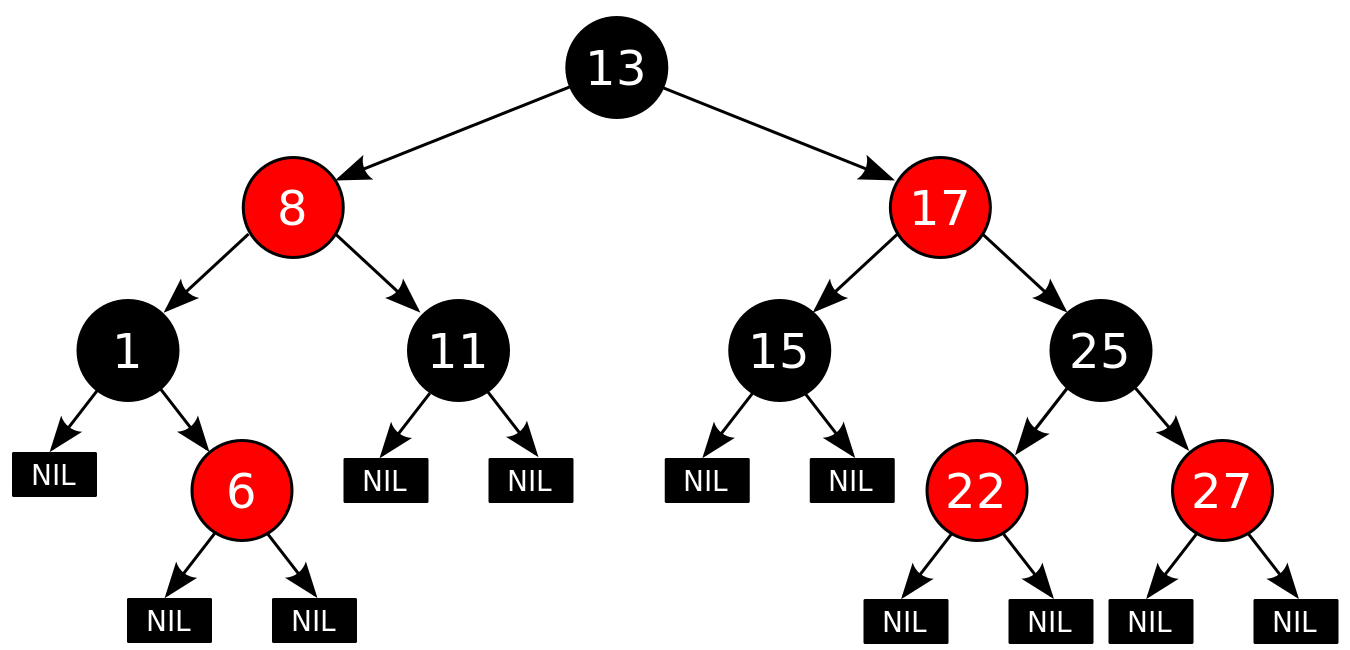
\includegraphics[width=\textwidth]{images/Red-black_tree_example}};

      \tikz[align=left] \node [below=of rbtree,node font=\tiny\itshape] {By Cburnett -- Own work, CC
        BY-SA 3.0\\https://commons.wikimedia.org/w/index.php?curid=1508398};
    \end{column}

    \begin{column}{.5\textwidth}<3->
      \setlength{\bytesize}{0.2cm}
      \setlength{\memwidth}{8\bytesize}
      \setlength{\memheight}{5cm}

      \begin{tikzpicture}[
          word/.style={
            draw=black!50,
            minimum height=\bytesize,
            minimum width=8\bytesize,
            inner sep=0pt
          },
          anchor=south west
        ]

        \node (word) at (0,0) [word,fill=blue!90!black,text=white] {\tiny value};
        \node (next) [word,above=0 of word,fill=red!90!black] {};
        \node (prev) [word,above=0 of next,fill=yellow!90!black] {};
        \node (parent) [word,above=0 of prev,fill=green!90!black] {};
        \node (color) [word,above=0 of parent,fill=black!20!white] {};
        \node [above left=0 and -\bytesize of parent,
          rectangle,
          inner sep=0pt,
          minimum width=\bytesize,
          minimum height=\bytesize,
          draw=black!50,
          fill=none,
          label={90:{\tiny color}}
        ] {};

        \node (wordp) [word,above right=1.1 and .1 of word,fill=blue!90!black,opacity=.3] {};
        \node (nextp) [word,above=0 of wordp,fill=red!90!black,opacity=.3] {};
        \node (prevp) [word,above=0 of nextp,fill=yellow!90!black,opacity=.3] {};
        \node (parentp) [word,above=0 of prevp,fill=green!90!black,opacity=.3] {};
        \node (colorp) [word,above=0 of parentp,fill=black!20!white,opacity=.3] {};

        \node (wordl) [word,below left=1.1 and .1 of word,fill=blue!90!black,opacity=.3] {};
        \node (nextl) [word,above=0 of wordl,fill=red!90!black,opacity=.3] {};
        \node (prevl) [word,above=0 of nextl,fill=yellow!90!black,opacity=.3] {};
        \node (parentl) [word,above=0 of prevl,fill=green!90!black,opacity=.3] {};
        \node (colorl) [word,above=0 of parentl,fill=black!20!white,opacity=.3] {};

        \node (wordr) [word,below right=1.1 and .1 of word,fill=blue!90!black,opacity=.3] {};
        \node (nextr) [word,above=0 of wordr,fill=red!90!black,opacity=.3] {};
        \node (prevr) [word,above=0 of nextr,fill=yellow!90!black,opacity=.3] {};
        \node (parentr) [word,above=0 of prevr,fill=green!90!black,opacity=.3] {};
        \node (colorr) [word,above=0 of parentr,fill=black!20!white,opacity=.3] {};

        \draw[{Circle[length=2pt]}-Stealth,black!80] (parent.east) to [out=0,in=270] node[auto,swap] {\tiny parent} (wordp.south);
        \draw[{Circle[length=2pt]}-Stealth,black!80] (prev.west) to [out=180,in=90] node[auto,swap] {\tiny left} (colorl.north);
        \draw[{Circle[length=2pt]}-Stealth,black!80] (next.east) to [out=0,in=90] node[auto,swap] {\tiny right} (colorr.north);

      \end{tikzpicture}
    \end{column}
  \end{columns}
\end{frame}

\begin{frame}{Hands-on}
  \begin{itemize}
  \item C++ $\rightarrow$ Containers
  \item Inspect, build and run \code{containers.cpp}, also using \code{perf}
  \item Extend it to manage an \code{std::list}
  \item Compare the performance obtained with the two containers
  \end{itemize}
\end{frame}

% !TeX root = cpp-esc22.tex

\section{Compile-time computation}

\begin{frame}{Doing things at compile-time}

  \begin{itemize}
  \item C++ has always been very strong in compile-time manipulation of program entities
  \item Thanks mainly to its support for templates
    \begin{columns}[T]
      \begin{column}{.1\textwidth}
      \end{column}
      \begin{column}{.2\textwidth}
        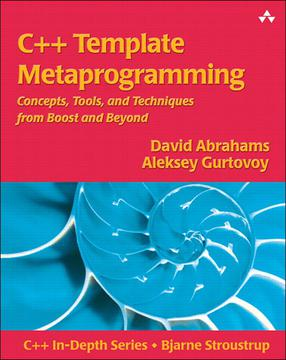
\includegraphics[width=\textwidth]{images/boost_mpl.jpeg}
      \end{column}
      \begin{column}{.2\textwidth}
        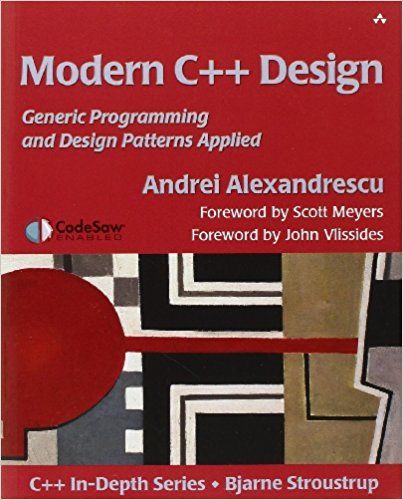
\includegraphics[width=\textwidth]{images/Modern_C++_Design.jpg}
      \end{column}
      \begin{column}{.2\textwidth}
      \end{column}
    \end{columns}
  \item Let's see two use cases
    \begin{itemize}
    \item Type introspection
    \item Computation
    \end{itemize}
  \end{itemize}

\end{frame}

\begin{frame}[fragile]{Type introspection}

  Query the type system to get information about types:
  \begin{itemize}
  \item how big is this type? {\small\code{sizeof(T)}}
  \item is this type default constructible? {\small\code{is\_default\_constructible\_v<T>}}
  \item is this type move-assignable? {\small\code{is\_move\_assignable\_v<T>}}
  \item can the move assignment throw? {\small\code{is\_nothrow\_move\_assignable\_v<T>}}
  \item are these two types the same? \small{\code{is\_same\_v<T1, T2>}}
  \item what's the common type for these types? {\small\code{common\_type\_t<int, unsigned, float>}}
  \end{itemize}

  \begin{codeblock}<2->{
template<typename T>
class uniform_real_distribution \{
  static_assert(std::is_floating_point_v<T>);
  \ddd
\};}\end{codeblock}

\end{frame}

\begin{frame}[fragile]{Iterator traits}

  \code{std::iterator\_traits} is a class template that provides
    properties about an iterator in terms of member types
    \begin{itemize}
    \item \code{\alert<3>{difference\_type}} is a signed integer to identify the
      distance between iterators
    \item \code{value\_type} is the type obtained dereferencing an iterator
    \item \code{pointer} is the type of pointer to \code{value\_type}
    \item \code{reference} is the type of reference to \code{value\_type}
    \item \code{\alert<3>{iterator\_category}} is one of input, output, forward,
      bidirectional, random-access
  \end{itemize}
  
  \begin{codeblock}<2->{
template<typename T>
struct iterator\_traits<T*> // specialization for a pointer
\{
  typedef random_access_iterator_tag iterator_category;
  typedef T                          value_type;
  typedef ptrdiff_t                  difference_type;
  typedef T*                         pointer;
  typedef T&                         reference;
\};}\end{codeblock}
\end{frame}

\begin{frame}[fragile]{Tag dispatching}
  \begin{codeblock}
\uncover<3->{template<class It>
\alt<8->{\alert<8>{auto}}{typename \alert<2>{iterator_traits<It>::difference_type}}
__distance(It first, It last\only<6->{, \alert<6-7>{random_access_iterator_tag} tag}) \{\only<3-5>{ // \alert<3>{for random-access iterators}}
  return last - first;
\}}

\uncover<4->{template<class It>
\alt<8->{\alert<8>{auto}}{typename \alert<2>{iterator_traits<It>::difference_type}}
__distance(It first, It last\only<6->{, \alert<6-7>{input_iterator_tag} tag}) \{\only<4-5>{ // \alert<4>{for input iterators}}
  typename iterator_traits<It>::difference_type n = 0;
  while (first != last) \{ ++first; ++n; \}
  return n;
\}}

template<class It>
\alt<8->{\alert<8>{auto}}{typename \alert<2>{iterator_traits<It>::difference_type}}
\alert<1>{distance}(It first, It last) \{
  \uncover<5->{return __distance(first, last\only<6->{, \alert<6>{iterator_traits<It>::category}\alert<7>{\{\}}});}\only<5>{ // which one?}
\}\end{codeblock}

\end{frame}

\begin{frame}[fragile]{Compile-time computation}

  \begin{itemize}
  \item
    Compute values to be used in contexts where a constant expression is required:
    \begin{itemize}
    \item boolean condition in a \code{static\_assert}
    \item size of an \code{std::array}
    \item \ldots
    \end{itemize}
  \item Statically initialize constant objects
  \item Reduce as much as possible the computation needed at runtime
  \item \ldots
  \end{itemize}

  \uncover<2->{Let's compute the factorial of a number at compile time}
\end{frame}

\begin{frame}[fragile]{Factorial with templates}

  Using a class template and non-type template parameters

  \begin{codeblock}
template<int N>
struct F        \uncover<3->{// general (recursive) case}
\{
  static const int value = \uncover<2->{N * F<N-1>::value};
\};

\uncover<3->{template<>
struct F<0>     // base case
\{
  static const int value = 1;
\};}

static_assert(F<5>::value == 120);
\uncover<4->{std::array<char, F<5>::value> buffer;}\end{codeblock}
\end{frame}

\begin{frame}[fragile]{Factorial with a function}

  Iterative function

  \begin{codeblock}
int factorial(int N) \{
  int r = 1;
  while (N > 0) \{ r *= N-{}-; \}
  return r;
\}\end{codeblock}

Recursive function

\begin{codeblock}
int factorial(int N) \{
  return N == 0 ? 1 : N * factorial(N-1);
\}\end{codeblock}

\begin{codeblock}<2->{
static_assert(\alert<2>{factorial(5)} == 120);    // error
std::array<char, \alert<2>{factorial(5)}> buffer; // error}\end{codeblock}

\end{frame}
\begin{frame}[fragile]{\texttt{constexpr}}

  \begin{itemize}[<+->]
  \item The \code{constexpr} specifier specifies that the value of a variable or
    function can appear in a constant expression
  \item The variable or the function can be evaluated at compile-time
  \item A function can be evaluated at compile-time only if the arguments are
    known at compile-time
    \begin{itemize}
    \item plus a few other constraints
    \end{itemize}
  \end{itemize}

  \begin{codeblock}<+->{
\alert{constexpr} int factorial(int N) \{ // iterative
  int r = 1;
  while (N > 0) \{ r *= N-{}-; \}
  return r;
\}

\alert{constexpr} int factorial(int N) \{ // recursive
  return N == 0 ? 1 : N * factorial(N-1);
\}

\uncover<3->{static_assert(factorial(5) == 120);}
\uncover<4->{\alert{constexpr} auto f5 = factorial(5);
std::array<char, f5> buffer;}}\end{codeblock}
\end{frame}

\begin{frame}[fragile]{\code{if constexpr}}

  Factorial using a function template with a \textit{constexpr-if}

  \begin{codeblock}<2->{
template<int N>
\alert<2>{constexpr} auto Factorial()
\{
  if constexpr (N > 0) \{
    return N * Factorial<N-1>();
  \} else \{
    return 1;
  \}
\}

\uncover<3->{static_assert(\alert<3>{Factorial<5>()} == 120);
constexpr auto f5 = \alert<3>{Factorial<5>()};
std::array<char, f5> buffer;}}\end{codeblock}
  
\end{frame}

\begin{frame}{Hands-on}
  \begin{itemize}
  \item Take the \code{pi} function in \code{pi\_time.cpp} and make it \code{constexpr}
  \item Implement a \code{constexpr} function that checks if a number is prime
  \item Take \code{containers\_assoc.cpp} and extend it to cover also the use of
    the \code{std::set} and \code{std::unordered\_set} associative containers.
    To fill the associative containers you can simply insert all the numbers
    from $0$ to $N$, without random generation and without advancing. In order
    to dispatch to the correct implementation you can use the
    \code{is\_associative} trait already included in that file, using it either
    as a tag or in a \textit{constexpr-if}.
  \item Construct a compile-time table corresponding to a
    \href{https://en.wikipedia.org/wiki/Pascal\%27s_triangle}{Pascal's Triangle}
    of N rows, where N is a compile-time constant.
  \end{itemize}
\end{frame}

% !TeX root = cpp-esc22.tex

\section{Additional material}

\section*{Type deduction}

\begin{frame}[fragile]{\texttt{auto}}
  Let the compiler deduce the type of a variable from the initializer

  \begin{codeblock}
\uncover<1->{auto i = 0;                // int
auto u = 0U;               // unsigned int
auto p = &i;               // int*
auto d = 1.;               // double
auto c = \upquote{a};              // char
auto s = "a";              // char const*}
\uncover<2->{auto t = std::string\{"a"\}; // std::string
std::vector<std::string> v;
auto it = std::begin(v);   // std::vector<std::string>::iterator}
\uncover<3->{using namespace std::chrono\_literals;
auto u = 1234us;           // std::chrono::microseconds}
\uncover<4->{auto e;                    // error}\end{codeblock}
\end{frame}

\begin{frame}[fragile]{\texttt{auto} and references}

  \begin{itemize}
  \item \texttt{auto} never deduces a reference
  \item if needed, \code{\&} must be added explicitly
  \end{itemize}

\begin{codeblock}
T v;

auto  v1 = v;     // T  -- v1 is a copy of v
auto\& v2 = v;     // T\& -- v2 is an alias of v
\alert{auto  v3 = v2;    // T  -- v2 is a copy of v}\end{codeblock}

\end{frame}

\begin{frame}[fragile]{\code{auto} and \code{const}}

  \begin{itemize}
  \item \code{auto} makes a mutable copy
  \item \code{auto const} (or \code{const auto}) makes a non-mutable copy
  \item \code{auto\&} preserves \code{const}-ness
  \end{itemize}

  \begin{codeblock}
T v;

auto        v1 = v; // T        -- v1 is a mutable copy of v
auto const  v2 = v; // T const  -- v2 is a non-mutable copy of v
auto\&       v3 = v; // \alert{T\&}       -- v3 is a \alert{mutable} alias of v
auto const\& v4 = v; // T const\& -- v4 is a non-mutable alias of v\end{codeblock}

  \begin{codeblock}
T const v;

auto        v1 = v; // T        -- v1 is a mutable copy of v
auto const  v2 = v; // T const  -- v2 is a non-mutable copy of v
auto\&       v3 = v; // \alert{T const\&} -- v3 is a \alert{non-mutable} alias of v
auto const\& v4 = v; // T const\& -- v4 is a non-mutable alias of v\end{codeblock}

\end{frame}

\begin{frame}[fragile]{How to check the deduced type?}
  \begin{itemize}
  \item Trick by S. Meyers
    \begin{codeblock}{
template<typename T> struct D;

auto k = 0U;
D<decltype(k)> d; // error: aggregate 'D<\alert{unsigned int}> d'...

auto const o = 0.;
D<decltype(o)> d; // error: aggregate 'D<\alert{const double}> d'...

auto const\& f = 0.f;
D<decltype(f)> d; // error: aggregate 'D<\alert{const float\&}> td'...

auto s = "hello";
D<decltype(s)> d; // error: aggregate 'D<\alert{const char*}> d'...

auto\& t = "hello";
D<decltype(t)> d; // error: aggregate 'D<\alert{const char (\&)[6]}> d'...}\end{codeblock}

  \item \code{decltype} returns the type of an expression
    \begin{itemize}
    \item at compile time
    \end{itemize}
  \end{itemize}
\end{frame}

\section*{More on lambda expressions}

\begin{frame}[fragile]{Lambda: closure}
  The evaluation of a lambda expression produces an unnamed function object (a
  \textit{closure})
  \begin{itemize}
  \item The \texttt{operator()} corresponds to the code of the body of the
    lambda expression
  \item The data members are the captured local variables
  \end{itemize}

  \begin{columns}[t]
    \begin{column}{.5\textwidth}
      \begin{codeblock}<2->{
\uncover<4-6>{int v = 3;}

\uncover<2->{auto l = [}\temporal<5-6>{}{=}{v = 3}\uncover<2->{]}\uncover<3->{(\alt<-7>{int }{auto} i)\uncover<9->{\alert<9>{ -> int}}
\{ return i + v; \}}

\uncover<6->{auto r = l(5); // 8}}\end{codeblock}

      \uncover<7>{}
    \end{column}

    \begin{column}{.5\textwidth}
      \begin{codeblock}<2->{
\uncover<2->{class SomeUniqueName \{
  \uncover<5->{int v\_;}
 public:
  \uncover<5->{explicit SomeUniqueName(int v)
    : v\_\{v\} \{\}}
  \uncover<8->{template<typename T>}
  \alt<-8>{auto}{\alert<9>{int }} operator()\uncover<3->{(\alt<-7>{int}{T  } i)
  \{ return i + v\uncover<5->{\_}; \}}
\};}

\uncover<4->{int v = 3;}
\uncover<2->{auto l = SomeUniqueName\{}\uncover<5->{v}\uncover<2->{\};}
\uncover<6->{auto r = l(5); // 8}}\end{codeblock}
    \end{column}
  \end{columns}
\end{frame}

\begin{frame}[fragile]{Lambda: capturing}

  \begin{itemize}
  \item Automatic variables used in the body need to be captured
    \begin{itemize}
    \item \texttt{[]} capture nothing
    \item \texttt{[=]} capture all by value
    \item \texttt{[k]} capture \texttt{k} by value
    \item \texttt{[\&]} capture all by reference
    \item \texttt{[\&k]} capture \texttt{k} by reference
    \item \texttt{[=, \&k]} capture all by value but \texttt{k} by reference
    \item \texttt{[\&, k]} capture all by reference but \texttt{k} by value
    \end{itemize}

    \begin{columns}[t]
      \begin{column}{.5\textwidth}
        \begin{codeblock}<2->{
int v = 3;
auto l = [\only<3->{\alert<3>{\&}}v] \{\};}\end{codeblock}
      \end{column}

      \begin{column}{.5\textwidth}
        \begin{codeblock}<2->{
class SomeUniqueName \{
  int\only<3->{\alert<3>{\&}} v\_;
 public:
  explicit SomeUniqueName(int\only<3->{\alert<3>{\&}} v)
    : v\_\{v\} \{\}
  \ddd
\};

auto l = SomeUniqueName\{v\};}\end{codeblock}
      \end{column}
    \end{columns}
  \item<4-> Global variables are available without being captured
  \end{itemize}
\end{frame}

\begin{frame}[fragile]{Lambda: \texttt{const} and \texttt{mutable}}
  \begin{itemize}
  \item By default the call to a lambda is \texttt{const}
    \begin{itemize}
    \item Variables captured by value are not modifiable
    \end{itemize}
  \item<2-> A lambda can be declared \texttt{mutable}
  \end{itemize}

  \begin{columns}
    \begin{column}{.5\textwidth}
      \begin{codeblock}<1->{
[]\only<2->{\alert<2>{() mutable}}\only<3->{\alert<3>{ -> void}} \{\};}\end{codeblock}
    \end{column}

    \begin{column}{.5\textwidth}
      \begin{codeblock}<1->{
struct SomeUniqueName \{
  \alt<-2>{auto}{\alert<3>{void}} operator()() \only<1>{\alert{const} }\{\}
\};}\end{codeblock}
    \end{column}
  \end{columns}

  \begin{itemize}
  \item<4-> Variables captured by reference can be modified
    \begin{itemize}
    \item There is no way to capture by \texttt{const\&}
    \end{itemize}
  \end{itemize}

  \begin{codeblock}<4->
int v = 3;
[\&v] \{ ++v; \}();
assert(v == 4);\end{codeblock}

\end{frame}

\begin{frame}[fragile]{Lambda: dangling reference}

  Be careful not to have dangling references in a closure
  \begin{itemize}
  \item It's similar to a function returning a reference to a local variable
  \end{itemize}

  \begin{codeblock}
auto make\_lambda()
\{
  int v = 3;
  return [\alert{&}] \{ return v; \}; // return a closure
\}

auto l = make\_lambda();
auto d = l(); // the captured variable is dangling here\end{codeblock}

  \begin{codeblock}
auto start\_in\_thread()
\{
  int v = 3;
  return std::async([\alert{&}] \{ return v; \});
\}\end{codeblock}

\end{frame}


\section*{More on move}

\begin{frame}[fragile]{Rvalue reference}
  \begin{itemize}
  \item A \textbf{\code{T\&\&}} is an rvalue reference
    \begin{itemize}
    \item introduced in C++11
    \end{itemize}
  \item It binds to rvalues but not to lvalues
  \end{itemize}

  \begin{codeblock}<2->{\tiny
class Thing;
Thing make\_thing();

Thing t;

\uncover<3->{Thing      &  r = t;}\uncover<4->{            // ok}
\uncover<5->{Thing      && r = t;}\uncover<6->{            // error}
\uncover<7->{Thing      &  r = make\_thing();}\uncover<8->{ // error}
\uncover<9->{Thing      && r = make\_thing();}\uncover<10->{ // ok}
\uncover<11->{Thing const&  r = make\_thing();}\uncover<12->{ // ok (!)}
\uncover<13->{Thing const&& r = make\_thing();}\uncover<14->{ // ok, but what for?}}\end{codeblock}

  \begin{codeblock}<15->{\tiny
class String \{
  // move constructor
  String(String\alert<15>{&&} tmp) : s\_(tmp.s\_) \{
    tmp.s\_ = nullptr;
  \}
\};

String s2\{s1\};           // call String::String(String const&)
String s3\{get\_string()\}; // call String::String(String&&)}\end{codeblock}

\end{frame}

\begin{frame}[fragile]{Rvalue reference \insertcontinuationtext}
  \begin{itemize}
  \item Any function can accept rvalue references
    \begin{codeblock}
void foo(String&&);

foo(get\_string());
foo(String\{"hello"\});\end{codeblock}
  \item lvalues can be explicitly transformed into rvalues
    \begin{codeblock}
String s;
foo(s);            // error
foo(std::move(s)); // ok, I don't care any more about s
s.size();          // dangerous\end{codeblock}
  \end{itemize}

\end{frame}

\begin{frame}[fragile]{Overloading on \&\&}
  \begin{itemize}
  \item<1-> A function can be overloaded for temporaries
    \begin{itemize}
    \item useful if there are significant opportunities of optimization
    \end{itemize}
    \begin{codeblock}{\tiny
void foo(Widget const&) \{\ddd\}
void foo(Widget&&) \{\ddd\}

Widget w\{\ddd\};
foo(w);           // calls foo(Widget const&)
foo(Widget\{\ddd\}); // calls foo(Widget&&)}\end{codeblock}
  \item<2-> For more than one parameter it becomes less desirable
    \begin{itemize}
    \item consider pass by value, if move is cheap
    \item especially useful for "sinks", e.g. in constructors
      \begin{codeblock}{\tiny
struct S \{
  T1 t1\_; T2 t2\_;
  S(T1 t1, T2 t2) : t1\_(std::move(t1)), t2\_(std::move(t2)) \{\ddd\}
\};

T1 t1; T2 t2;
S s\{t1, make\_t2()\};
S s\{make\_t1(), t2\};}\end{codeblock}
    \end{itemize}
  \end{itemize}
\end{frame}
\begin{frame}[fragile]{Copy operations}

  \begin{codeblock}{\tiny
class Widget \{
  \ddd
  Widget(Widget const& other);
  Widget& operator=(Widget const& other);
\};}\end{codeblock}

  \begin{description}[<2->]
  \item [copy constructor] Allows the \alert{construction} of an object as a copy of another object

    \begin{codeblock}<.->{\tiny
Widget w1;
Widget w2\{w1\};}\end{codeblock}

  \item [copy assignment] Allows to change the value of an \alert{existing} object as a copy of another object

    \begin{codeblock}<.->{\tiny
Widget w1, w2;
w2 = w1;}\end{codeblock}

  \end{description}

  \begin{itemize}[<3->]
  \item The two objects are/remain distinct
  \item The copied-from object is not changed
  \item After the copy the two objects should compare equal
  \end{itemize}

\end{frame}

\begin{frame}[fragile]{Move operations}

  \begin{codeblock}{\tiny
class Widget \{
  \ddd
  Widget(Widget&& other);
  Widget& operator=(Widget&& other);
\};}\end{codeblock}

  \begin{description}[<2->]
  \item [move constructor] Allows the \alert{construction} of an object stealing
    the internals of another object

    \begin{codeblock}<.->{\tiny
Widget w\{make\_widget()\};}\end{codeblock}

  \item [move assignment] Allows to change the value of an \alert{existing}
    object stealing the internals of another object

    \begin{codeblock}<.->{\tiny
Widget w;
w = make\_widget();}\end{codeblock}

  \end{description}

  \begin{itemize}[<3->]
  \item The two objects are/remain distinct
  \item The moved-from object is usually changed
    \begin{itemize}[<*>]
    \item to a \textit{valid but unspecified} state
    \item it must be at least destructible and possibly reassignable
    \end{itemize}
  \end{itemize}

\end{frame}

\begin{frame}[fragile]{On move}
  \begin{itemize}
  \item<1-> A move is typically cheaper than a copy, but it can be as expensive
  \item<2-> If the \textit{Return Value Optimization} is not applied, the return
    value of a function is moved, not copied, into destination
  \item<3-> \code{operator=(T\&\&)} can assume that the argument is a temporary,
    hence different from \code{this}
    \begin{itemize}
    \item There is no need to check for self-assignment
    \item But be sure that in such event there is no crash
    \item Rule of thumb: \code{std::swap} must work

      \begin{codeblock}
template<typename T>
void swap(T& a, T& b) \{
  T t\{std::move(a)\};
  a = std::move(b);
  b = std::move(t);
\}\end{codeblock}

    \end{itemize}
  \end{itemize}
\end{frame}

\begin{frame}[fragile]{\code{= default}}
  \begin{itemize}
  \item Explicitly tell the compiler to generate a \underline{special member
    function} according to the default implementation
  \end{itemize}

  \begin{codeblock}<2->
class Widget \{
  int i = 0;
 public:
  Widget(Widget const&);
  \uncover<3->{Widget() \alert<3>{= default};}
\};

\uncover<2->{static\_assert(std::is\_copy\_constructible<Widget>::value);}
\uncover<2->{static\_assert(\only<2>{!}std::is\_default\_constructible<Widget>::value);}\end{codeblock}

\end{frame}

\begin{frame}[fragile]{\code{= delete}}

  \begin{itemize}
  \item<1-> A function can be declared as \textit{deleted}, marking it with
    \mbox{\alert{= delete}}
  \item<2-> For example, a class can be made \alert{non copyable} deleting its
    copy operations
  \item<3-> Calling a deleted functions causes a compilation error
  \item<5-> Any function can be deleted
  \end{itemize}

  \begin{codeblock}<1->
template<typename P>
class SmartPointer \{
  \ddd
  \textbf<3>{SmartPointer(SmartPointer const&) \alert<1>{= delete};}
  \textbf<4>{SmartPointer& operator=(SmartPointer const&) \alert<1>{= delete};}
\};

\uncover<2->{using SPI = SmartPointer<int>;

static\_assert(!std::is\_copy\_constructible<SPI>::value);
static\_assert(!std::is\_copy\_assignable<SPI>::value);}

\uncover<3->{SPI sp1, sp2;}
\uncover<3->{SPI sp3\{sp1\}; // error}
\uncover<4->{sp2 = sp1;    // error}\end{codeblock}

\end{frame}

\section*{Error management}

\begin{frame}{Mechanisms for error management}

  \centering\alert{The sooner the errors are identified, the better}

  \begin{itemize}
  \item \texttt{static\_assert}
    \begin{itemize}
    \item Logical assertion that must be valid at \underline{compile time}
    \end{itemize}
  \item \texttt{assert}
    \begin{itemize}
    \item Logical assertion that must be valid at \underline{run time}
    \end{itemize}
  \item Exceptions
    \begin{itemize}
    \item To express an error condition happening at \underline{run time},
      typically related to a lack of resource
    \end{itemize}
    \item \color[rgb]{.6,.6,.6}{C-style error codes}
      \begin{itemize}
      \item \color[rgb]{.6,.6,.6}{They can be ignored (but they should not!)}
      \end{itemize}
    \item \ldots
  \end{itemize}
\end{frame}

\begin{frame}[fragile]{\texttt{static\_assert}}
  Check that a certain constant boolean expression is satisfied during
  compilation
  \begin{itemize}
  \item If not, fail compilation with the specified message
  \end{itemize}

  \begin{codeblock}<2->{
#include <type\_traits>

struct C \{
  C(C const\&) = default;
  C\& operator=(C const\&) = delete;
\};

\alert<2-3>{static\_assert(!std::is\_default\_constructible<C>::value, "");
static\_assert( std::is\_copy\_constructible\_v<C>);
static\_assert(!std::is\_copy\_assignable\_v<C>);
static\_assert( std::is\_\only<3->{nothrow\_}move\_constructible\_v<C>);
static\_assert(!std::is\_move\_assignable\_v<C>);
static\_assert( std::is\_destructible\_v<C>);
static\_assert(sizeof(C) == 1);}}\end{codeblock}

  \uncover<4->{
    A static assertion declaration can appear practically anywhere
    \begin{itemize}
    \item There is no effect, hence no overhead, at run time
    \end{itemize}
  }
\end{frame}

\begin{frame}[fragile]{\texttt{assert}}

  Check that a certain boolean expression is satisfied at run time
  \begin{itemize}
  \item If not satisfied, it means that the state of the program is corrupted
    $\rightarrow$ better to close the program as soon as possible (calling
    \code{std::abort})
  \end{itemize}

  \begin{codeblock}<2->{
template<class T> class Vector \{
  T* p;
  \ddd
  T\& operator[](int n) \{
    \uncover<3->{\alert{assert(p != nullptr);         // class invariant (sort of)}}
    \uncover<4->{\alert{assert(n >= 0 \&\& n < size()); // function pre-condition}}
    return p[n];
  \}
\};}\end{codeblock}

  \uncover<5->{
    Useful during testing/debugging
    \begin{itemize}
    \item Can be disabled for performance reasons (\texttt{-DNDEBUG})
    \item Avoid side effects in \texttt{assert}s
    \end{itemize}
  }
\end{frame}

\begin{frame}[fragile]{Exceptions}

  \begin{itemize}
  \item Mechanism to report errors out of a function, stopping its execution
  \item Useful to express \textit{post-conditions}
  \item Help separate application logic from error management
  \end{itemize}

  \begin{codeblock}<2->{
class Thing \{\ddd\};
\uncover<5->{class Exception \{\ddd\};}

auto make\_thing() \{
  \uncover<3->{auto res = acquire\_resources\_to\_build\_thing();}
  \uncover<4->{if (!success(res)) \{}
    \uncover<5-6>{Exception e\{\ddd\};}
    \uncover<5->{throw \alt<-6>{e}{Exception\{\ddd\}};}
  \uncover<4->{\}}
  return Thing\{\uncover<3->{res}\}; \uncover<6->{// not executed in case of exception}
\}}\end{codeblock}

  \uncover<8->{Note that all local variables (e.g. \texttt{res}) are properly
    destroyed when exiting the function, be it via \texttt{return} or via
    \texttt{throw}}
\end{frame}

\begin{frame}[fragile]{Exception propagation}

  \begin{columns}[t]

    \begin{column}{.5\textwidth}
      \begin{codeblock}
\uncover<1->{auto high() \{}
\uncover<9->{  try \{}
\uncover<2->{    // this part is executed}
\uncover<1->{    mid();}
\uncover<10->{    // this part is not executed}
\uncover<9->{  \} catch (E\alert<12>{\&} e) \{}\uncover<12->{ // \alert<12>{by reference}}
\uncover<11->{    // use e}
\uncover<9->{  \}}
\uncover<1->{\}}

\uncover<1->{auto mid() \{}
\uncover<3->{  T t; // this part is executed}
\uncover<1->{  low();}
\uncover<7->{  // this part is not executed}
\uncover<8->{  // \alert<8>{T is properly destroyed}}
\uncover<1->{\}}

\uncover<1->{auto low() \{}
\uncover<4->{  // this part is executed}
\uncover<5->{  throw E\{\};}
\uncover<6->{  // this part is not executed}
\uncover<1->{\}}\end{codeblock}
    \end{column}

    \begin{column}<13->{.5\textwidth}
      \begin{itemize}
      \item An exception is propagated up the stack of function calls until a
        suitable catch clause is found
      \item If no suitable catch clause is found the program is
        \texttt{terminate}d
      \item During stack unwinding all automatic objects are properly destroyed
        \begin{itemize}
        \item Remember smart pointers!
        \end{itemize}
      \end{itemize}
    \end{column}

  \end{columns}
\end{frame}

\begin{frame}{Exception safety}

  Different levels of safety guarantees (for member functions):

  \begin{description}
  \item [basic] If an exception is thrown, no resource is leaked and the object
    is left in a \textit{valid but unspecified} state
    \begin{itemize}
    \item the object should be at least safely assignable and destroyable
    \item every class should provide at least the basic guarantee
    \end{itemize}
  \item [strong] Transaction semantics: if an exception is thrown, the object's
    state is as it was before the function was called
  \item [no-throw] The operation is always successful and no exception leaves
    the function
  \end{description}

\end{frame}

\begin{frame}[fragile]{\texttt{noexcept}}

  \begin{itemize}
  \item A function can be declared \texttt{noexcept}, telling the compiler that
    the function
    \begin{itemize}
    \item doesn't throw, or
    \item<2-> is not able to manage exceptions \uncover<3->{$\rightarrow$ better
      \texttt{terminate}}
    \end{itemize}

    \begin{codeblock}<4->{
class Handle \{
  Handle(Handle\&\& o) \alert{noexcept} : \ddd \{ \ddd \}
  \ddd
\};}\end{codeblock}

  \item<5-> Declaring functions (not only member functions) \texttt{noexcept} helps
    the compiler to optimize the code
  \item<5-> If move operations, especially the constructor, are \texttt{noexcept} the
    compiler/library can apply \textbf{significant} optimizations
    \begin{itemize}
    \item E.g. in order to provide the strong guarantee
      \texttt{std::vector::push\_back} must copy, not move, objects, if the move
      can throw
    \end{itemize}
  \end{itemize}

\end{frame}

\begin{frame}{Move and \texttt{noexcept}}
  \begin{itemize}
  \item<1-> \texttt{T\& T::operator=(T\&\& tmp)} is typically easy to make
    \texttt{noexcept}
    \begin{itemize}
    \item<2-> Rely on the \texttt{noexcept}-ness of data members' move-assignments
    \end{itemize}
  \item<3-> \texttt{T::T(T\&\& tmp)} may be more difficult
    \begin{itemize}
    \item<3-> Start with one object (\texttt{tmp}), end up with two (\texttt{*this}
      and \texttt{tmp})
    \item<4-> Can rely on \texttt{T::T()} being \texttt{noexcept} as well
    \item<4-> Which is not obvious if a resource has to be acquired
    \end{itemize}
  \end{itemize}
\end{frame}

\begin{frame}[fragile]{Destructor and \texttt{noexcept}}

  \begin{itemize}
  \item The destructor is by default \texttt{noexcept}
    \begin{itemize}
    \item i.e. releasing a resource should not fail
    \end{itemize}
  \item<2-> Don't do anything overly complicated in the destructor or swallow all
    exceptions locally
  \end{itemize}

  \begin{codeblock}<3->
class Thing \{
  ~Thing()
  \{
    try \{
      \vdots
    \} catch (\alert{...}) \{ // catch \alert{all} exceptions
      // e.g. log something, provided logging doesn't throw
    \}
  \}
\};\end{codeblock}

  \begin{itemize}
  \item<4-> It's always possible to declare a destructor, like any other function,
    \texttt{noexcept(false)}
  \end{itemize}

\end{frame}


\end{document}
